
\documentclass[12pt]{article}

\usepackage{amssymb,amsmath,amsfonts,eurosym,geometry,ulem,graphicx,caption,color,setspace,sectsty,comment,footmisc,caption,pdflscape,subfig,array,hyperref,booktabs,multirow,rotating}
\usepackage[round]{natbib}

\hypersetup{
	colorlinks=true,
	citecolor=blue,
	linkcolor=red,
	filecolor=magenta,      
	urlcolor=cyan,
}

\setlength{\bibsep}{20pt}

\onehalfspacing
\newtheorem{theorem}{Theorem}
\newtheorem{corollary}[theorem]{Corollary}
\newtheorem{proposition}{Proposition}
\newenvironment{proof}[1][Proof]{\noindent\textbf{#1.} }{\ \rule{0.5em}{0.5em}}
\newtheorem{definition}{Definition}

\newtheorem{hyp}{Hypothesis}
\newtheorem{subhyp}{Hypothesis}[hyp]
\renewcommand{\thesubhyp}{\thehyp\alph{subhyp}}

\newcommand{\red}[1]{{\color{red} #1}}
\newcommand{\blue}[1]{{\color{blue} #1}}

\newcolumntype{L}[1]{>{\raggedright\let\newline\\arraybackslash\hspace{0pt}}m{#1}}
\newcolumntype{C}[1]{>{\centering\let\newline\\arraybackslash\hspace{0pt}}m{#1}}
\newcolumntype{R}[1]{>{\raggedleft\let\newline\\arraybackslash\hspace{0pt}}m{#1}}

\geometry{left=1.0in,right=1.0in,top=1.0in,bottom=1.0in}

\newcommand{\source}[1]{\caption*{Source: {#1}} }
\newcommand{\note}[1]{\caption*{Note: {#1}} }

\begin{document}

\begin{titlepage}
\title{The Sex Ratio, Marriage and Bargaining: \\ A Look at China} %\thanks{abc}}
\author{Francisco Javier Rodr\'iguez Rom\'an \thanks{I thank Matthias Kredler for his excellent guidance and support as my main advisor. I have benefited from conversations with Andr\'es Erosa, Luisa Fuster, Felix Wellschmied, Bel\'en Jerez, Juanjo Dolado, William Fuchs, Ana Moreno, Michelangelo Rossi, Rub\'en Veiga, Elizaveta Pronkina, Ismael G\'alvez, Beatriz Gonz\'alez, Onursal Bagirgan and Tom\'as Rodr\'iguez at Carlos III. I received helpful feedback at the XXIV Workshop on Dynamic Macroeconomics in Vigo and at the Macroeconomics Seminar at University of Mannheim, especially from \'Arpad \'Abrah\'am, Juan Carlos Conesa, Tim Kehoe, Victor R\'ios-Rull, Andreas Guylas, Anne Hannusch, Lei Li, Mich\`ele Tertilt, Minchul Yum, Efi Adamopoulou, Sena Coskun and Husnu Dalgic. All errors or shortcomings are my own.} \\
		Universidad Carlos III de Madrid \\
		%Office 15.1.14 \\
		%Calle Madrid 126, 28903 \\
		%Getafe, Spain \\
		%+34 622925412 \\
		\href{mailto:frarodri@eco.uc3m.es}{frarodri@eco.uc3m.es}}
\date{}
\maketitle
\begin{abstract}
\noindent  
This paper quantifies the importance of changes in the sex ratio on married couples' paid work, housework, leisure and marital sorting on education. To do so, I develop a model of marriage, bargaining and time allocation, and calibrate it to data for China, a country that has experienced a surge in boy births relative to girls' since the 1980s. I perform a decomposition exercise and find that the change in the sex ratio explains up to one half of the decrease in married women's paid work and half of the increase in their leisure time between 1990 and 2010, as well as one fifth of the increase in assortative mating. Moreover, in the model the changes in the sex ratio affect time allocation mainly through bargaining within the household and very marginally via marital sorting. \\
\vspace{0in}\\
\noindent\textbf{Keywords:} Sex ratio, China, marriage, bargaining, female labor supply \\
\vspace{0in}\\
\noindent\textbf{JEL Codes:} J11, J12\\

\bigskip
\end{abstract}
\setcounter{page}{0}
\thispagestyle{empty}
\end{titlepage}
\pagebreak \newpage


%\doublespacing


\section{Introduction} \label{sec:introduction}

Between 1990 and 2010, weekly hours devoted to paid work and to housework decreased by 14\% and 47\% respectively among young (20 to 35 years old) married women in China, while paid work remained constant and housework decreased much less for their male counterparts. As a result, the female-to-male leisure ratio for young married people increased. For singles however this ratio remained constant. 

This paper studies how changes in the sex ratio could be partly responsible for these trends. One of the most striking instances of the sex ratio deviating from its natural level has been going on in China since the 1980s. Census data paints a clear picture of an increasing gap between the number of males and females. Table \ref{srb_census} shows the sex ratio at birth for the last four census years. It goes up from an already somewhat high 1.085 boys per girl in 1982 to almost 1.2 in 2010. Naturally this imbalance does not have an immediate impact the marriage market, but does so 20 to 30 years ahead, when people in those cohorts start getting married. 

In Figure, \ref{sex_ratio_20_30} I project the data from the 2000 census both backward and forward to obtain sex ratios for marriageable-age population (individuals aged 20 to 35 years old)\footnote{The reader might notice that the sex ratios at birth are higher than the sex ratios for the marriageable age population 20 years later up to 2000. 
%I discuss intercensal inconsistencies and other issues around the measurement of the sex ratio in Appendix \ref{sec:sexratioappendix}. 
There are intercensal inconsistencies with and other issues around the measurement of the sex ratio. However, although there is disagreement on the real scale of the imbalance in the sex ratio, it seems clear that an increase has indeed occurred: ``the recorded sex imbalance is not a statistical artifact, but a reality'', see \citealp{cai13}.}. As can be observed, there was an increase between 1990 and 2010, and the imbalance is going to keep widening all the way to 2020.    

\begin{table}[htbp]
	\centering
	\caption{Sex ratio at birth (male births over female births), 1982-2010}
	\begin{tabular}{lr}
		\toprule
		Year & \multicolumn{1}{l}{Sex ratio at birth} \\
		\midrule
		1982 & 1.085 \\
		1990 & 1.113 \\
		2000 & 1.169 \\
		2010 & 1.179 \\
		\bottomrule
		\bottomrule
	\end{tabular}
	\label{srb_census}
	\source{Tabulation on the Population Census of the People's Republic of China, National Bureau of Statistics.}
\end{table}

\begin{figure}[]
	\centering
	\caption{Sex ratio in China for population aged 20-35, 1990-2020}
	\includegraphics[width=.6\textwidth]{sex_ratio_20_35}
	\label{sex_ratio_20_30}
	\source{Projected from the 2000 Population Census.}
\end{figure}

The underlying causes of China's skewed sex ratio at birth, although fascinating in their own right, are not explored in this paper. I take the demographics as exogenous and focus instead on analyzing the effects that the men surplus has on marriage market outcomes and the allocation of resources by couples within the household.

Conditions in the marriage market affect the outside option of getting married. If the sex ratio goes up, the value of remaining single for a woman increases, as she is more likely to meet potential spouses, while the opposite is true for men. That means that the bargaining position of women improves when negotiating the allocation of resources within marriage. Moreover, the sex ratio affects the types of households that are formed, i.e. the degree of assortative mating and female/male hypergamy (when females/males marry a spouse of a higher status then themselves), as women become choosier-and men less so-when there is an excess of males.

To study the mechanisms mentioned above, I develop a model that allows for agents to be heterogeneous based on their education. I divide people into three skill groups according to their education attainment: low (primary or less), medium (high school) and high (college). Moreover, in the model marriage decisions are endogenous and bargaining between spouses determines resource allocation. The bargaining positions of women and men depend on the conditions in the marriage market. 

To avoid tractability problems that emerge when studying two-sided search models with heterogeneous agents, while keeping marital sorting endogenous, I structure marriage markets in two stages. People may meet potential spouses of different types at the beginning of their life as singles, while in subsequent periods they only meet people of their own type. This is as an extension of the structure used in \cite{fernandezetal05}. In terms of time allocation, the model works in a very similar fashion as the one in \cite{knowles13}. People allocate time between three competing uses: paid work, housework, and leisure. Through paid work households generate resources to purchase a private consumption good and home equipment. A combination of the latter and housework time yields a home-produced good. Married households decide via bargaining on how to allocate time and split the private consumption good. As mentioned earlier, the sex ratio affects the decisions of married couples as it increases the outside value of wives.

I calibrate the model so that in steady-state equilibrium the time allocation and marital sorting moments match their data counterparts for China in 1990. Indeed, the model is able to reproduce the data almost perfectly for that year. Next I change the sex ratio, the distribution of people across skill groups, the wage structure, and the parameters associated to home production one at a time to their 2010 values. The model does a good job replicating qualitatively the changes in time allocation and marital sorting that occurred between 1990 and 2010. In the model, as in the data, paid work time decreases and leisure increases for married women, while the time allocation does not change very much for married men. The degree of assortative mating increases both in the model and in the data, although more so in the latter. 

A decomposition exercise reveals that the increase in the sex ratio alone accounts for 38\%-52\%\footnote{The percentages of the changes that are explained by the sex ratio are given as ranges because the model is not linear and therefore the results vary with the order of the decomposition. This is discussed more in depth in section \ref{sec:quant}.} of the decrease in paid work time and for 26\%-47\% of the increase in leisure for married women between 1990 and 2010. Moreover, it accounts for 18\%-61\% of the increase in assortative mating. Decomposing further the effect of the sex ratio on married people's time allocation, I find that most of it operates via bargaining, and very little of it through the changes in marital sorting (different households being formed as a result of the excess men in the marriage market).

As the skill distribution changed substantially between 1990 and 2010, the effects of the changes in the sex ratio were not felt equally among all skill groups. In the model, the sex ratio among singles in steady state equilibrium increased the most between 1990 and 2010 for low and medium-skilled people, while actually decreased for the high skilled ones. This happened for two reasons. First, the skill distribution became more equal across genders, with the fraction of women with high skill actually overcoming that of men's in 2010. Second, the fact that it is quite common that women marry men with higher skill than themselves (while the opposite is very rare) means that women in the marriage markets face competition from women with lower skill levels. Similarly, men face competition from higher skilled men. Therefore, when the sex ratio increases, more women marry up and more men marry down. However, that is not possible for women in the highest skill group and for men in the lowest. In the model, women in the first two skill groups experience the largest decrease in paid work and increase in leisure.

Finally, the model implies that the increase in the sex ratio leads to 7\%-10\% higher private consumption for married women, at the expense of a decrease for married men of 4.5\%-8.5\%.

This paper contributes to several lines of research. First, the literature on marriage. Economists have been interested in it since the seminal work by \cite{becker73,becker74}. Within the marriage markets literature, one strand may be described as a general equilibrium approach as in \cite{chiapporiweiss06}, and the other as the search frictions approach, as in \cite{greenwoodetal16}. The model developed here belongs to the latter. Moreover, this paper speaks to the growing literature on the importance of intra-household bargaining on aggregate outcomes, in which \cite{knowles13} is a prominent example, and a forerunner of this paper. My main contribution to this literature is that I study steady state equilibria with heterogeneous agents, while the literature in general avoids having both at the same time. 

Second, the paper adds to the substantial literature that explores the effect sex ratios have on various socioeconomic outcomes. Most of these papers are empirical and employ reduced-form specifications to capture local effects. A classic example is \cite{angrist02}. He exploits the variation in sex ratios among different ethnic groups of immigrants in the United States, and finds that higher sex ratios increase the likelihood of marriage and decrease the labor force participation of females. \cite{grosjeankhattar19} report similar findings for Australia, where sex ratios were heavily male-biased historically as a result of the British policy of sending convicts there during the 19th century. Moreover, they find that the effect is persistent, i.e. women work fewer hours outside the house in areas where the sex ratio was more male-biased, even today with a normal sex ratio. \cite{abramitzkyetal11} present evidence on the improvement of the position of males in the marriage market due to their relative scarcity due to WWII in France. In regions where male mortality was higher the marriage rates went up for men and down for women. In addition, males in those areas were less likely to marry females of lower social classes. For the case of China, \cite{weizhang11} explore the hypothesis that the rising sex ratio in China creates a competitive savings motive for parents with a son, increasing the household savings rate. 

Two papers stand at the intersection of marriage literature and the socioeconomic effects of variations in the sex ratio. \cite{seitz09} develops a dynamic model of marriage and labor force participation to assess the extent to which differences in those outcomes between blacks and whites in the United States are due to lower sex ratios among the former. There are however some important differences between the approach in that paper and mine. On one hand, \cite{seitz09} has the advantage of having a detailed panel data set to estimate the structural parameters of her model. On the other hand, I rely on a calibration strategy using aggregate moments. Moreover, by comparing two populations, \cite{seitz09} has the advantage of being able to use the current and future sex ratios of whites when performing counterfactual exercises for blacks. I do not have an obvious way of pinning down expectations on future sex ratios in my counterfactual exercises, which generates an important additional challenge.

\cite{wang18} provides a quantitative model with imbalanced sex ratios, marriage, divorce and intra-household bargaining in China. The main result is on welfare: females are 9.5\% better off in consumption units and men are 14.42\% worse due to the high sex ratio. There are also some important differences between this paper and mine. First, the author does not include housework in the model, as I do. This is important, since a reduction in paid work does not mean that married women are enjoying more leisure. Secondly, the two-sided search model with heterogeneous agents in that paper features endogenous expectations about the distribution of education among singles, which make the model's equilibrium properties hard to assess. In my paper I avoid this with the two-stage marriage markets discussed earlier. Incidentally, this structure allows me to better capture the marital sorting patterns.

The rest of the paper is organized as follows. Section \ref{sec:dataandfacts} discusses the data and lays out some facts about relevant changes that China experienced during the two decades between 1990 and 2010. Section \ref{sec:model} is devoted to describe the model. In section \ref{sec:calibration}, I explain the calibration strategy and showcase the model fit. Section \ref{sec:quant} is devoted to the decomposition and counterfactual exercises and its results. Section \ref{sec:conclusions} concludes.    

\section{Data and empirical facts} \label{sec:dataandfacts}

For this section and the rest of the paper, I rely mainly on the various waves of the China Health and Nutrition Survey (CHNS)\footnote{The CHNS is an international collaborative project between the Carolina Population Center at the University of  North Carolina at Chapel Hill and the National Institute for Nutrition and Health at the Chinese Center for Disease Control and Prevention.} and the findings of \cite{getao14} on the changes in China's wage structure. A detailed description of the data can be found on appendix \ref{sec:dataappendix}.

In what follows I present a series of empirical facts for China between the years 1990 and 2010. These facts concern changes in time allocation, distribution of skills, wages and assortative mating. I focus on people aged 20-35 years old, what I call the marriageable age, as they are the ones that are primarily affected by the changes in the sex ratio during this period.   

In Figure \ref{fig:time_use_married}, I plot the time devoted to paid work and to housework\footnote{For a detailed explanation of how I construct the data for housework see Appendix \ref{sec:dataappendix}.} by married people. Several things stand out. First, women spend less time doing both paid work and housework in 2010 than in 1990. This means that their leisure time must have increased. Second, men's paid work and housework are quite similar in 1990 and 2010. Moreover, the time trend for both is quite flat. Therefore, leisure time for married men has remained roughly constant during the period. These changes imply that the female-to-male ratio of paid work and housework has decreased, while it has increased for leisure. This ratio, on the other hand, remained constant among single people, as shown in Figure \ref{fig:leisure_ratio}. 

\begin{figure}[hp]
	\centering
	\caption{Time allocation for Chinese married people aged 20-35, 1990-2010}\label{fig:time_use_married}
	\subfloat[Paid work]{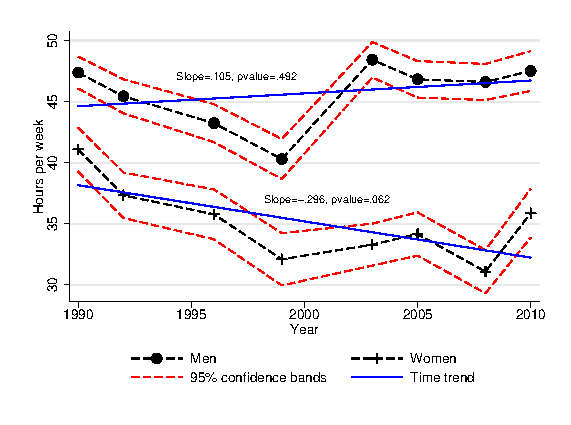
\includegraphics[width=.6\textwidth]{paid_work_time}}
	\\
	\subfloat[Housework]{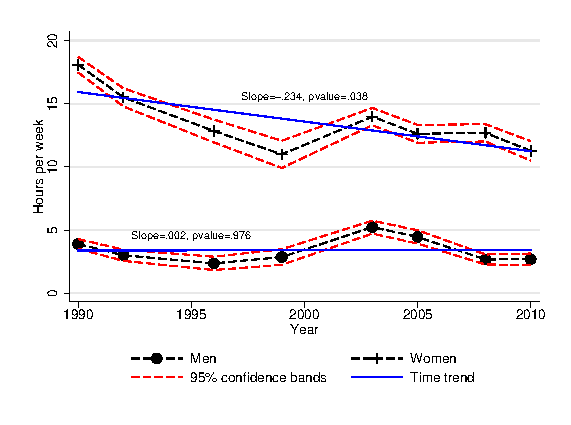
\includegraphics[width=.6\textwidth]{housework_time}}
	\source{Author's calculations using the China Health and Nutrition Survey.}
\end{figure}

\begin{figure}[hp]
	\centering
	\caption{Female-to-male leisure ratio for population aged 20-35, 1990-2020}
	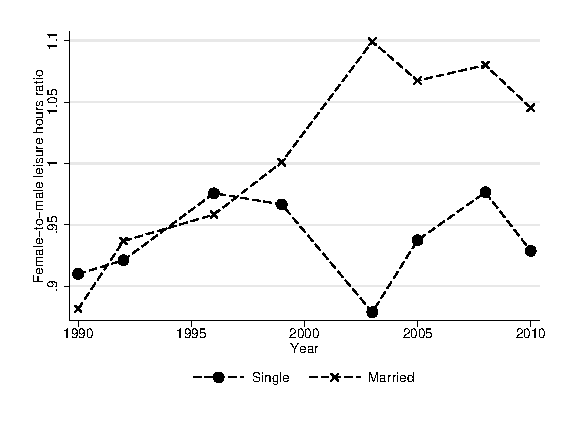
\includegraphics[width=.6\textwidth]{leisure_ratio_all}
	\label{fig:leisure_ratio}
	\source{Author's calculations using the China Health and Nutrition Survey.}
\end{figure}

The skill distribution based on educational attainment registers important changes between 1990 and 2010. Figure \ref{fig:skill_dist} shows those changes. For both men and women, there has been an increase in the fraction of high skilled. However, it was steeper for women. While in 1990 4.47\% of men and only 3.69\% of women were classified as high skill, the percentages were 28.5\% and 31.0\% respectively in 2010. That is, women surpassed men in college attainment. At the same time, the fraction of low skilled went down for both genders. In 1990, 32.8\% of men and 46.9\% of women fell in this category. By 2010, the percentages had fallen to 13.6\% and 17.8\%. Looking at the relative proportions it becomes apparent that the reduction was steeper for women. In 1990, the relative fraction of low skilled women to men was 1.42, while in 2010 it was 1.30. Finally, the fraction of medium skill people fell for men and rose for women. 

An identical analysis finds single people

\begin{figure}[hp]
	\centering
	\caption{Skill distribution for Chinese people aged 20-35, 1990-2010}\label{fig:skill_dist}
	\subfloat[Males]{\includegraphics[width=.6\textwidth]{skill_dist_male}}
	\\
	\subfloat[Females]{\includegraphics[width=.6\textwidth]{skill_dist_female}}
	\source{Author's calculations using the China Health and Nutrition Survey.}
	\note{skill levels are defined based on educational attainment (highest grade attained). Low skill individuals are those with primary or less, medium skill are those with middle-high school and high skill those with some college or more.}
\end{figure}

In terms of wages, dramatic changes occurred in the two decades between 1990 and 2010. It is well known that after the Opening of China that started with Deng Xiaoping's reforms in 1978, China has seen spectacular economic growth. According to the International Monetary Fund, GDP per capita rose on average 8.95\% per year between 1980 and 2010 and by 9.58\% between 1990 and 2010\footnote{Growth rate of Gross Domestic Product per capita, constant prices in 2011 international dollars (PPA adjusted) as reported in the World Economic Outlook Database, October 2018.}. This growth has translated into quite large wage gains, although some groups benefited more than others.

I present the changes in China's wage structure by skill and sex in Table \ref{tab:wage_struct_ge_tao}\footnote{For a more in depth discussion of the data in \cite{getao14} and some of my own estimates on the changes in the wage structure using the CHNS data, see Appendix \ref{sec:dataappendix}.}. Overall, the growth in wages has followed closely GDP per capita growth. However, medium and high skilled wages grew faster than low skilled, leading to an increase in the skill premium. Moreover, male wages grew faster than female's. In 1992, the gender wage ratio (female over male wages) was 0.83, but in 2007 it had fallen to 0.75. 

\begin{table}[htbp]
	\centering
	\caption{Changes in wage structure in China, 1992-1997}
	\begin{tabular}{lrrr}
		\toprule
		& \multicolumn{1}{c}{Annual growth} & \multicolumn{2}{c}{Premium} \\
		\cmidrule{3-4}Classification & \multicolumn{1}{c}{1992-1997} & 1992  & 1997 \\
		\midrule
		Overall & 7.6\% &   -    & - \\
		&       &       &  \\
		By skill &       &       &  \\
		Low   & 5.9\% &   -    & - \\
		Medium & 6.9\% & 6.44\% & 22.46\% \\
		High  & 8.5\% & 28.63\% & 86.08\% \\
		&       &       &  \\
		By sex &       &       &  \\
		Female & 7.2\% &   -    & - \\
		Male  & 7.9\% & 20.01\% & 33.04\% \\
		\bottomrule
		\bottomrule
	\end{tabular}
	\label{tab:wage_struct_ge_tao}
	\source{Author's calculations using the data presented in Table 1 of \cite{getao14}.}
	\note{skill premium is calculated with respect to low skill wages. The gender wage premium is calculated with respect to female wages.}
\end{table}

Finally, I use three different methods to measure assortative mating, based on \cite{greenwoodetal14}\footnote{For a detailed explanation of how I construct the three measures, see Appendix \ref{sec:dataappendix}.}. I present the results in Figure \ref{fig:assortative_mating}. For the three measures considered, a higher value means more assortative mating, and for all of them the values for 2010 are higher than for 1990. Therefore, it seems that assortative mating rose in China among young people during the period of interest.

\begin{figure}[]
	\centering
	\caption{Assortative mating in China among people aged 20-35, 1990-2010}\label{fig:assortative_mating}
	\subfloat[Regression approach]{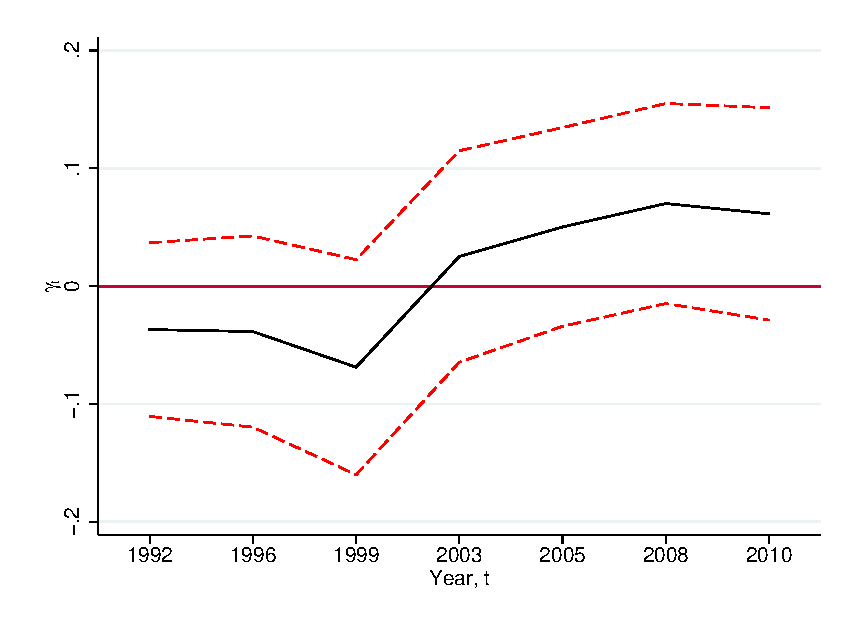
\includegraphics[width=.5\textwidth]{gammas}}
	\\
	\subfloat[Rank correlation approach]{\includegraphics[width=.5\textwidth]{kendallstau}}
	\\
	\subfloat[Contingency table approach]{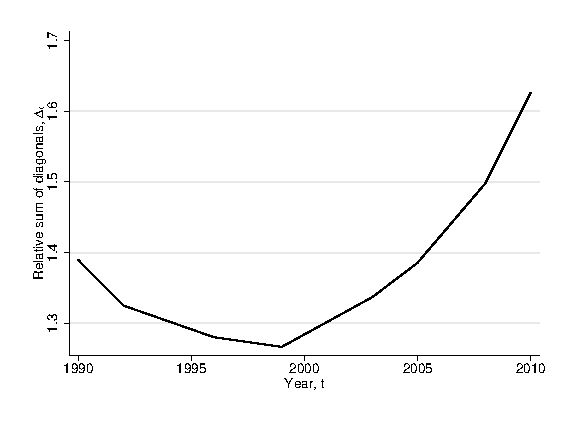
\includegraphics[width=.5\textwidth]{deltas}}
	\source{Author's calculations using the China Health and Nutrition Survey.}
	\note{For panel a, the dashed lines represent 95\% confidence intervales. These are not available for panels b and c.}
\end{figure}

%The IPUMS 1\% sample of the Chinese censuses of 1982, 1990 and 2000 are a main source for demographic information, although they contain no information on income. Moreover, the 2010 census micro data is unfortunately not avaliable anywhere. Only the official tabulation provided by the National Bureau of Statistics of China is accessible. For detailed income, employment and time use information, I draw upon the various waves of the China Health and Nutrition Survey (CHNS) of the UNC Carolina Population Center, and a paper by \cite{getao14}. 

%For this section and the rest of the paper, I rely on various data sources. The IPUMS 1\% sample of the Chinese censuses of 1982, 1990 and 2000 are a main source for demographic information, although they contain no information on income. Moreover, the 2010 census micro data is unfortunately not avaliable anywhere. Only the official tabulation provided by the National Bureau of Statistics of China is accessible. For detailed income, employment and time use information, I draw upon the various waves of the China Health and Nutrition Survey (CHNS) of the UNC Carolina Population Center, and a paper by \cite{getao14}. 

%Accounting for China's sex ratio is no straightforward task. There are intercensal inconsistencies in the size of male and female cohorts, especially those born between 1981 and 1990, which are key cohorts in these study. Moreover the lack of micro data for the 2010 census means this numbers cannot be corroborated by researchers. Concretely, the sex ratios are too low to be plausible given the sex ratio at birth. \cite{cai13} explores the possibility of the census inconsistencies being attributable to underreporting of girl births. However, when he compares census, \textit{hukou}\footnote{China's national household registration system} and primary school enrolment data, he concludes that this cannot explain more than a quarter of the drop in the sex ratio for the cohorts born between 1981 and 1990. Therefore, I mainly use data on the sex ratio at birth to estimate the magnitude of the sex ratio for each cohort.

%Figure \ref{lfp} shows how female labor force participation in China dropped by slightly more than 15 percentage points between 1990 and 2010. On the intensive margin, average hours worked per year also fell from 2000 per year to 1600. If we look at these changes by marital status, as shown in figure \ref{lfp_marst}, it becomes clear that they are concentrated among married women, which is hardly surprising considering that the experience for other countries is that big changes in female labor supply are mainly driven by this group.

%However, paid work is not the only kind of work people do. Has the decrease in hours worked outside home by married women been accompanied by a corresponding increase in housework? Figure \ref*{fig:time_use_married} answers this question: no. In fact, housework time has decreased for women and remained roughly constant for men.
 
%Figure \ref*{fig:time_use_married} shows the evolution of paid work and housework for young married people between 1990 and 2010. 

%This begs the question of what has been going on with wages. The Opening of China that started with Deng Xiaoping's reforms in 1978 has led to spectacular economic growth. According to the International Monetary Fund, GDP per capita rose on average by 8.95\% per year between 1980 and 2010 and by 9.58\% between 1990 and 2010\footnote{Growth rate of Gross Domestic Product per capita, constant prices in 2011 international dollars (PPA adjusted) as reported in the World Economic Outlook Database, October 2018}. 

%Using the CHNS data on income, I estimate that for both men and women, there was a seven-fold increase in the real average wage per hour between 1990 and 2010, for an average growth rate of around 10\% per year, and that the gender wage ratio remained close to 0.75 and didn't change significantly, as shown in figure \ref{fig:gender_wage_ratio}. However, a study by \cite{getao14} finds lower wage growth (a three-fold increase, approximately), and a falling gender wage ratio. Their study uses a sample of the Urban Household Surveys (UHS), which the authors claim to be high quality, and that was unavailable to researchers before. On the one hand, income data in this survey is of greater quality than the CHNS data. On the other hand, the gender wage ratio I estimate is conditional on education, age and province, which may be more relevant to this study, while theirs is not and may be driven by composition effects that are of no interest in this paper.

%\begin{figure}
%	\centering
%	\caption{Gender wage ratio in China, 1990-2010}\label{fig:gender_wage_ratio}
%	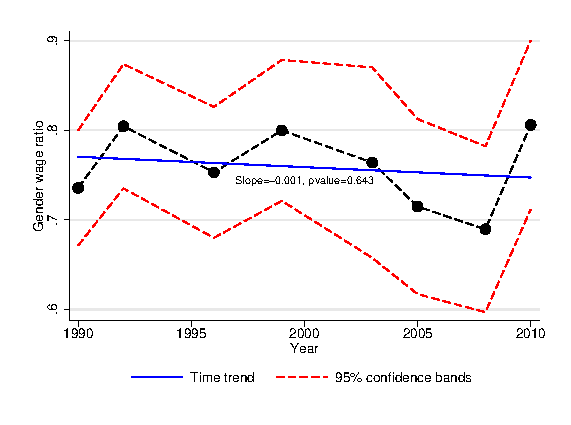
\includegraphics[width=.6\textwidth]{gender_wage_ratio}
%	\source{Author's calculations using the China Health and Nutrition Survey}
%\end{figure}
%
%In any case, it would be hard to explain the developments on married couples' time allocation with via changes in relative wages between men and women. If the relative wages of women were falling, the standard unitary household model would predict that married women should substitute paid work with housework. If it were raising, it would predict the opposite. There is no scenario under which both paid work and housework fall in response to changes in the gender wage ratio.
%
%Another relevant change that occured in China during the period I'm interested is the increase in inequality. Figure \ref{fig:gini_hourly_wages_1990_2010} reports the Gini index for the real hourly wage for both men and women in the CHNS, which has gone up greatly. One of the drivers of this is the increase in the skill premium. As can be observed in figure \ref{fig:skill_premium}, in 1990 there was no discernible skill premium, while in 2010 it is significant for all education levels above primary.

%\begin{figure}[]
%	\centering
%	\caption{Real hourly wage inequality by sex in China, 1990-2010}\label{fig:gini_hourly_wages_1990_2010}
%	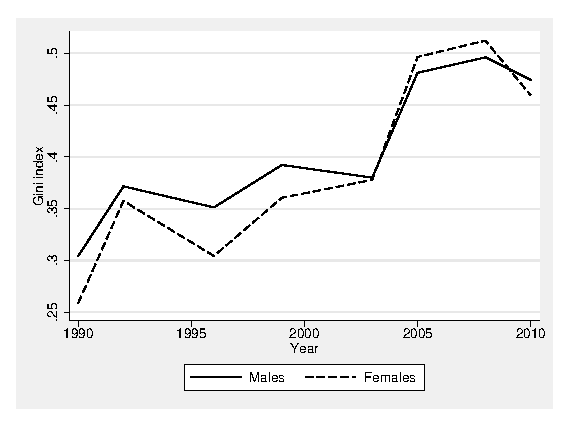
\includegraphics[width=.6\textwidth]{gini_real_hourly_wage_1990_2010}
%	\source{Author's calculations using the China Health and Nutrition Survey}
%\end{figure}
%
%\begin{figure}[]
%	\centering
%	\caption{Skill premium, 1990 and 2010}\label{fig:skill_premium}
%	\subfloat[Women]{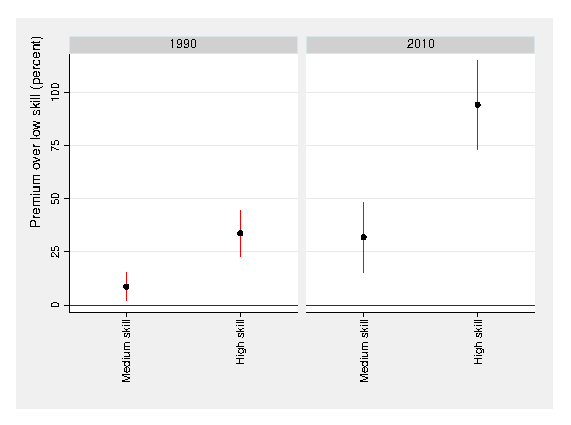
\includegraphics[width=.6\textwidth]{skill_premium_women}}
%	\\
%	\subfloat[Men]{\includegraphics[width=.6\textwidth]{skill_premium_men}}
%	\source{Author's calculations using the China Health and Nutrition Survey}
%\end{figure}
%
%Individual inequality in earnings potential may be amplified or reduced when aggregating household income by the degree of assortative mating. To assess how marital sorting has changed in China I use the three different measures found in \cite{greenwoodetal14}. First, I regress wife's education level on her husband's:
%
%\begin{align*}
%EDU_{my}^w = \alpha + \beta\times EDU_{my}^h+\sum_{t\in T} \gamma_t\times EDU_{my}^h\times YEAR_{ty}+\sum_{t\in T}\theta_t\times YEAR_{ty}+\epsilon_{my}
%\end{align*}
%
%In the specification above, $EDU_{mw}^y$ and $EDU_{mh}^y$ represent wife's and husband's years of education in marriage $m$ and year $y$, and $YEAR_{ty}$ is a time dummy that takes the value of 1 when $t=y$ and 0 otherwise, whith $T = \{1992,1996,1999,2003,2005,2008,2010\}$. The coefficient $\beta$ measures the correlation between wife's and husband's education in the base year (1990), the $\theta_t$'s control for the secular rise in education. I am interested in the $\gamma_t$'s which measure the difference between wife and husband's correlation in year $t$ and the baseline year. If $\gamma_t$ rises with $t$, there's evidence of increasing assortative mating over time.
%
%For the next two measures, I collapse the levels of education into five categories: no schooling (NS), primary (P), lower middle school (LM), upper middle school (UM) and college (C).
%
%The second measure of assortative mating I use is Kendall's $\tau$ rank correlation. A value of 1 means perfect positive rank correlation, that is, the man with the highest education level is married with the woman with the highest education level, the man with the second highest education level is married with the woman with the second highest education level and so forth. A value of -1 means the opposite, i.e perfect negative rank correlation. The closer Kendall's $\tau$ is to 1, the higher the assortative mating. I measure $\tau_t$ for $t\in \{1990,1992,1996,1999,2003,2005,2008,2010\}$. Again, if $\tau_t$ rises with $t$, this points to increasing assortative mating over time.
%


%\begin{table}[htbp]
%	\centering
%	\caption{Contingency table: assortative mating in 1990}
%	\begin{tabular}{lrrrrrrrrrr}
%		\toprule
%		\multicolumn{1}{c}{\multirow{2}[1]{*}{Wife}} & \multicolumn{10}{c}{Husband} \\
%		& \multicolumn{2}{c}{NS} & \multicolumn{2}{c}{P} & \multicolumn{2}{c}{LM} & \multicolumn{2}{c}{UM} & \multicolumn{2}{c}{C} \\
%		NS & \textbf{0.073} & \textbf{0.030} & 0.087 & 0.063 & 0.090 & 0.120 & 0.032 & 0.059 & 0.002 & 0.013 \\
%		P & 0.017 & 0.023 & \textbf{0.073} & \textbf{0.048} & 0.090 & 0.092 & 0.034 & 0.045 & 0.004 & 0.010 \\
%		LM & 0.012 & 0.033 & 0.045 & 0.069 & \textbf{0.174} & \textbf{0.132} & 0.074 & 0.065 & 0.009 & 0.014 \\
%		UM & 0.004 & 0.016 & 0.013 & 0.034 & 0.062 & 0.065 & \textbf{0.061} & \textbf{0.032} & 0.014 & 0.007 \\
%		C & 0.000 & 0.003 & 0.001 & 0.006 & 0.003 & 0.012 & 0.008 & 0.006 & \textbf{0.017} & \textbf{0.001} \\
%		\bottomrule
%	\end{tabular}
%	\label{tab:cont_tab_1990}
%	\source{Author's calculations using the China Health and Nutrition Survey}
%\end{table}
%
%
%Figure \ref{fig:assortative_mating} shows the results obtained with the three measures. The picture is quite clear: there has been an increase in assortative mating between 1990 and 2010.
%
%\begin{figure}[]
%	\centering
%	\caption{Assortative mating in China among people aged 20-35, 1990-2010}\label{fig:assortative_mating}
%	\subfloat[Regression approach]{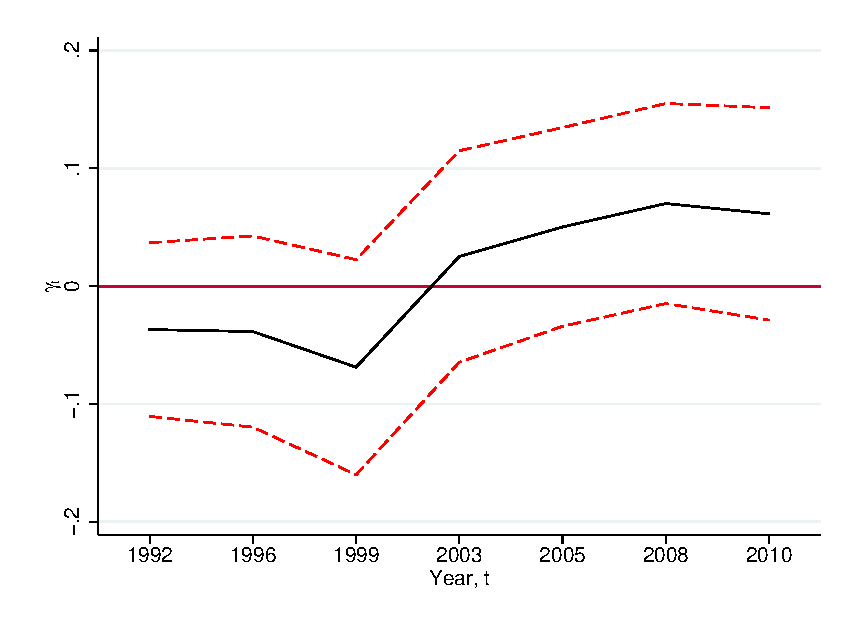
\includegraphics[width=.5\textwidth]{gammas}}
%	\\
%	\subfloat[Rank correlation approach]{\includegraphics[width=.5\textwidth]{kendallstau}}
%	\\
%	\subfloat[Contingency table approach]{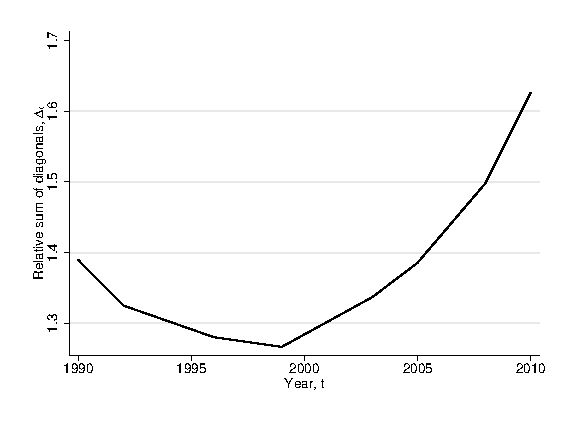
\includegraphics[width=.5\textwidth]{deltas}}
%	\source{Author's calculations using the China Health and Nutrition Survey}
%\end{figure}
%
%A number of questions arise after examining the data. Can the rising sex ratios explain the changes in time allocation among married couples, and hence the downward trend in female labor supply? Does an increase in the sex ratio augment or mitigate assortative mating? A larger sex ratio means better marriage opportunities for women. Moreover, if the gap in earnings potential among forming couples increases, women would be incentivized to work less hours outside and more inside the house. Can we extract conclusions about the underlying distribution of household resources between couples? A quantitative model of marriage, bargaining and time allocation can help address this issues.

\section{The Model} \label{sec:model}

It is hard to rationalize the time allocation patterns among married people under a unitary household framework. A decrease in the gender wage ratio would imply that women substitute paid work with housework, and men do the opposite. This means that the female to male paid work ratio decreases, while the housework ratio increases. In the data we observe that they both decrease. Moreover, wealth effects stemming from the rapidly rising wages combined with growing productivity in home production\footnote{\cite{greenwoodetal05} argue that what they call the revolution of consumer durable during the XXth century was an important factor in liberating women's time devoted to housework in the United States. Many of these durable goods became widely available in China much more recently than in the U.S.} can account for the increasing leisure that married women enjoy, but would also imply increasing leisure for men.    

Moreover, as suggested by the results in \cite{abramitzkyetal11}, the sex ratio may affect marital sorting. Assortative mating increased in China between 1990 and 2010. Was the rise in the sex ratio partially responsible for that? Or alternatively, would assortative mating had increased even more if the sex ratio had remained constant? 

To understand the effect the sex ratio has on resource allocation and marital sorting, it would be useful to have a model featuring a marriage market with search frictions (people have difficulties contacting potential spouses), bargaining within households, time allocation, and home production decisions. The search frictions imply that the sex ratio affects the probability of finding a viable spouse, which in turn affects the outside value of marriage (remaining single), the bargaining position of spouses and ultimately the resource allocation (including time). 

However, two-sided search models with heterogeneous agents are known to be intractable. The origin of this intractability is expectations: since the distribution of skills among single people is endogenous, agents need to form expectations about this multi-dimensional object in the future that affect their behavior today. The properties of the equilibrium, whether it exists and whether it is unique\footnote{\cite{burdettcoles97} describe the issue of multiplicity of steady-state equilibria in a two-sided search model under fully rational expectations and random search. Essentially, the cause is the presence of a sorting externality, which may lead to steady-state equilibria with distributions of singles that have more or less mass at the top of the distribution. The intuition goes as follows: suppose different types of agents can be arranged from most to least desirable, and that every agent agrees on this ordering (as is the case with skill). If those at the top of the distribution expect an abundance (paucity) of agents at the top on the other side, they will be more (less) selective, thus spending more time searching and generating the expected abundance (paucity). Moreover, this effect cascades down the distribution of types in complex ways. When an agent expects those on top of her to be more (less) selective, there are two opposing effects on her own selectiveness. On one hand, the probability of meeting someone with a higher type increases (decreases). On the other, conditional on meeting, the probability of that agent wanting to marry them decreases (increases).} are uncertain, not to mention the properties of a potential steady-state.

A common workaround for this issue is the assumption that whenever a couple gets married, two identical agents flow into singlehood to replace them. However, it implies that the primitives of the model are the distribution over types and sex ratio \textit{among singles}, not in the general population. This is problematic for my case since I am interested in generating counterfactual steady-state equilibria featuring different sex ratios among the general population. 

The structure of marriage markets I propose deals with this issue. Young agents that enter the marriage market are matched randomly with potential partners of any skill level. However, in subsequent periods they may only meet potential partners with the same skill as themselves. Therefore, agents face a trade-off between accepting matches with high quality but low earnings potential. This is inspired by \citet{fernandezetal05}. Agents therefore do not need to form expectations about the skill distribution among singles, which is the source of intractability. The model however, allows agents to marry outside of their skill level, meaning that marital sorting is still endogenous. 

Moreover, single and married households must allocate their time between paid work (which allows for consumption of market goods), housework (which allows for home production), and leisure (which generates utility directly). A combination of inputs for home production must also be chosen. The allocation of resources within married households responds to conditions in the marriage market, notably the sex ratio, via bargaining.
  
\subsection{The Setup}

The economy is populated by agents that are characterized by a gender $i\in \{f,m\}$ (female or male). At the time agents start looking for a spouse, they are also characterized by a type $z \in \mathcal{Z}$ that remains constant throughout their life. 

Time is discrete and infinite. All agents discount the future at a rate $\beta$ and face a constant probability of dying equal to $\delta$. Exogenous measures of 1 of females and $\theta_0$ of men enter the economy every period to replace those who die. Therefore, the overall measures of females and males in the general population are $\frac{1}{\delta}$ and $\frac{\theta_0}{\delta}$. Moreover, the sex ratio among entrants and in the general population is $\theta_0$. Finally, the probability distributions over types for each sex, $\mathcal{P}_i(z):z\in\mathcal{Z}\to\mathbb{R}^+$, $\sum_{z\in \mathcal{Z}}\mathcal{P}_i(z)=1$ for $i\in\{f,m\}$, are also exogenous.

\subsection{The time allocation and home production problem}

In every period, households need to decide how to allocate their time and how to produce home goods. The problem is almost identical to the one in \citet{knowles13}. Each agent is endowed with one unit of time that has to be allocated across leisure $l$, paid work $n$, and housework $h$. Thus, the time constraint for each agent is

\begin{align*}
	l+n+h=1.
\end{align*}

Utility over leisure, consumption of market and home goods takes a CES form:

\begin{align*}
	u\left(c,l,g\right) = \frac{\sigma_c}{1-\sigma}c^{1-\sigma}+\frac{\sigma_l}{1-\sigma}l^{1-\sigma}+\frac{\sigma_g}{1-\sigma}g^{1-\sigma}.
\end{align*}

The home production function is a Cobb-Douglas that takes as inputs housework time $h$ and home equipment $e_q$:

\begin{align*}
	G\left(h,e_q\right) = A_G\left[e_q^{1-\alpha_G}\right]h^{\alpha_G}.
\end{align*}

For the case of married couples, effective housework time $h$ is a function of wife's ($h_f$) and husband's ($h_m$) individual housework times:

\begin{align*}
	H(h_f,h_m)=\left[\eta_f h_f^{1-\eta}+\left(1-\eta_f\right)h_m^{1-\eta}\right]^{\frac{1}{1-\eta}}.
\end{align*}

\subsection{Wages and the price of home equipment}

Wages are an exogenous function of an agent's type and sex, which we denote as $\omega_i\left(z\right):\mathcal{Z}_i\to \mathbb{R}$ for $i\in\{f,m\}$. The price of home equipment is also an exogenous parameter denoted by $p_e$.

\subsection{Solution to the time allocation and home production problem}

Since there are no savings decisions and home equipment is a jump variable, the time allocation and home production problem is static. 

\subsubsection{Singles}

The indirect utility flow of a single person of sex $i$ and type $z$ is

\begin{align}
	U_i^S\left(z;p_e,\omega_i(z)\right) = & \max_{c,l,h,n,e_q,g} u\left(c,l,g\right) \label{eq:singletaprob} \\
	& \text{subject to} \nonumber \\
	& l+n+h = 1 \nonumber \\
	& g = G\left(h,e_q\right) \nonumber \\
	& c = \omega_i\left(z\right)n-p_e e_q. \nonumber
\end{align}

The closed-form demand functions for market goods, leisure and home produced goods are given by

\begin{align*}
	\left[c_i(z),l_i(z),g_i(z)\right] = \left[\left(\frac{\sigma_c}{\lambda_i(z)}\right)^{\frac{1}{\sigma}},\left(\frac{\sigma_l}{\lambda_i(z)\omega_i(z)}\right)^{\frac{1}{\sigma}},\left(\frac{\sigma_g}{\lambda_i(z) D_i(z)}\right)^{\frac{1}{\sigma}}\right],
\end{align*}

while the inputs for home production are proportional to $g_i(z)$:

\begin{align*}
	\left[h_i(z),e_{qi}(z)\right] = \left[\frac{g_i(z)}{x^g_i(z)}, \frac{x^e_i(z) g_i(z)}{x^g_i(z)}\right],
\end{align*}

where $\lambda_i(z)$ is the Lagrange multiplier associated to the budget constraint, $D_i(z)$ is the effective marginal price of home-produced goods, $x^e_i(z)$ is the ratio of home equipment to housework  and $x^g_i(z)$ is the ratio of of home production to housework. Closed-form expressions for these objects are derived in Appendix \ref{sec:timeallocationappendix}. 

In steady state, I denote the indirect utility associated to the problem in \ref{eq:singletaprob} just by $U_i^S\left(z\right)$.

\subsubsection{Married households}

The allocations for married households are the outcome of an auxiliary problem that finds the allocation on the Pareto frontier, taking as given the Pareto weight associated to the wife's utility $\chi_f$\footnote{The Pareto weight for the wife may vary with the wife and husband education types, but to save in notation we just denote it by $\chi_f$ instead of $\chi_f\left(z_f,z_m\right)$.} (and thus the one associated to the husband's utility, $1-\chi_f$). This weight is the result of bargaining, and thus responds to the conditions in the marriage market (in particular, to the sex ratio) in a way that I explain further down this section.   

Married households therefore maximize a welfare function that consists of a weighted sum of the utilities of each spouse. The problem faced by a married household with wife's type $z_f$ and husband's type $z_m$ is therefore:

\begin{align}
	& \max_{c_f,c_m,l_f,l_m,h_m,h_f,n_f,n_m,e_q,g} \left\lbrace \chi_f u_f\left(c_f,l_f,g\right)+\left(1-\chi_f\right) u_m\left(c_m,l_m,g\right) \right\rbrace \label{eq:marriedtaprob} \\
	& \text{subject to} \nonumber \\
	& l_f+h_f+n_f = 1 \nonumber \\
	& l_m+h_m+n_m = 1 \nonumber \\
	& h = H\left(h_f,h_m\right) \nonumber \\
	& g = G\left(h,e_q\right) \nonumber \\
	& c_m+c_f = \omega_f(z_f)n_f+\omega_m(z_m)n_m-p_e e_q. \nonumber
\end{align}

The closed form demands for market goods, leisure and home production are

\begin{align*}
	& \left[c_i(z_f,z_m,\chi_f),l_i(z_f,z_m,\chi_f),g(z_f,z_m,\chi_f)\right] = \\ & \left[ \left(\frac{\chi_f \sigma_c}{\lambda(z_f,z_m,\chi_f)}\right)^{\frac{1}{\sigma}}, \left(\frac{\left(1-\chi_f\right)\sigma_l}{\lambda(z_f,z_m,\chi_f)\omega_i(z_i)}\right)^{\frac{1}{\sigma}},\left(\frac{\sigma_g}{\lambda(z_f,z_m,\chi_f) D(z_f,z_m,\chi_f)}\right)^{\frac{1}{\sigma}}   \right]
\end{align*}

for $i\in\{f,m\}$ and $\chi_m = 1-\chi_f$. Home production inputs again are proportional to $g(z_f,z_m,\chi_f)$:

\begin{align*}
	&\left[h_f(z_f,z_m,\chi_f),h_m(z_f,z_m,\chi_f),e_q(z_f,z_m,\chi_f)\right] = \\ & \left[\frac{x^f(z_f,z_m,\chi_f)g(z_f,z_m,\chi_f)}{x^g(z_f,z_m,\chi_f)},\frac{g(z_f,z_m,\chi_f)}{x^g(z_f,z_m,\chi_f)},\frac{x^e(z_f,z_m,\chi_f)g(z_f,z_m,\chi_f)}{x^g(z_f,z_m,\chi_f)}\right].
\end{align*}

Closed-form expressions for $\lambda(z_f,z_m,\chi_f)$, $D(z_f,z_m,\chi_f)$, $x^g(z_f,z_m,\chi_f)$, $x^e(z_f,z_m,\chi_f)$, $x^f(z_f,z_m,\chi_f)$ are derived in Appendix \ref{sec:timeallocationappendix}.

I denote the indirect utility flow accrued by an agent of sex $i$ in a marriage of type $\left(z_f,z_m\right)$ with Pareto weights $\left(\chi_f,1-\chi_f\right)$ by $U_i^M\left(z_f,z_m,\chi_f;\omega_f(z_m),\omega_f(z_f),p_e\right)$. That is, the value of the above problem in \ref{eq:marriedtaprob} is given by

\begin{align*}
	\chi_f U_f^M\left(z_f,z_m,\chi_f;\omega_f(z_m),\omega_f(z_f),p_e\right)+\left(1-\chi_f\right) U_m^M\left(z_f,z_m,\chi_f;\omega_f(z_m),\omega_f(z_f),p_e\right).
\end{align*}

In steady state I denote these indirect utility flows just by $U_i^M\left(z_f,z_m,\chi_f\right)$ for $i\in\{f,m\}$.

\subsection{Marriage markets}

Agents may participate in two marriage markets in the model. The first one is a pooled market, in which they only stay for one period upon entry. In this market, they may meet randomly one agent of the opposite sex and of any skill level. All single agents that are not entrants participate in segregated markets in which they may only meet agents of the opposite sex and same skill level. They may participate in this markets for several periods. That is, agents may only marry someone with a different type upon entry.  

I will first describe the functioning of the same-skill marriage markets, and then how the pooled market.

\subsubsection{Marriage markets for same-skill agents}

Agents face search frictions when looking for potential spouses. Denote by $S_f(z)$, $S_m(z)$ and $\theta_{S}(z) = \frac{S_m(z)}{S_f(z)}$ the measures of females, males and the sex ratio among singles of type $z\in\mathcal{Z}$, respectively. In each period, single agents meet at most one agent of the opposite sex and the same type, where the measure of meetings is given by

\begin{align*}
X = \min \left\lbrace A_X S_m(z)^{\alpha_X} S_f(z)^{1-\alpha_X},S_f(z),S_m(z) \right\rbrace,
\end{align*}

and thus the probabilities of meeting a potential spouse are obtained dividing $X(z)$ by $S_i(z)$ for $i\in\{f,m\}$:

\begin{align*}
\pi_{i}\left(\theta_{S}(z)\right) = \begin{cases}
\min \left\lbrace A_X\left(\frac{1}{\theta_{S}(z)}\right)^{1-\alpha_X},1, \frac{1}{\theta_{S}(z)} \right\rbrace & \text{ if } i=m, \\
\min \left\lbrace A_X\theta_{S}(z)^{\alpha_X}, \theta_{S}(z),  1 \right\rbrace & \text{ if } i=f.
\end{cases}
\end{align*}

Upon meeting a potential spouse, agents draw a match quality $q$ from a distribution with cdf $Q_{z,z}$. This represents the flow value of companionship that each partner will enjoy during the marriage. After observing $q$, agents must decide whether they want to get married. 

Since the values of $q$ is constant, and in steady-state so are the wages $\omega_i(z)$ for $i\in\{f,m\}$ and price of home equipment $p_e$, in steady-state equilibrium there is no divorce. Moreover, I assume that if either partner dies, the other dies as well (there are no widowers). Therefore the value of a marriage between agents of type $z\in \mathcal{Z}$ for an agent of sex $i\in\{f,m\}$ and a given Pareto weight is

\begin{align}
	V_i^M\left(z,z,\chi_f,q\right)=\sum_{t=0}^{\infty}\left[\beta\left(1-\delta\right)\right]^t\left[U_i^M(z,z,\chi_f)+q\right]=  \frac{U_i^M(z,z,\chi_f)+q}{1-\beta\left(1-\delta\right)}. \label{eq:val_married}
\end{align}

Single agents face a probability of leaving the marriage market and become lifelong singles of $\rho$. This means that people can expect to spend on average $\frac{1}{\rho}$ periods being eligible for marriage. Moreover, it ensures that the sex ratio among singles does not explode due to the accumulation of men that were unlucky for many periods\footnote{The age difference among spouses doesn't change much in the data, staying close to 2 years.}. Apart from the utility derived from private goods consumption, leisure and the consumption of home-produced goods that results from solving problem \ref{eq:singletaprob}, single agents experience a fixed utility flow per period $\psi_i$. This represents an intrinsic value of being single. Note that $\psi_i$ could be negative. The value of remaining single in steady-state is thus

\begin{align*}
&V_i^S\left(z,\theta_{S}^E(z)\right) = U_i^S\left(z\right)+\psi_i+\beta\left(1-\delta\right)\left\lbrace \rho \frac{U_i^S\left(z\right)+\psi_i}{1-\beta\left(1-\delta\right)}+\right.\\ &\left.\left(1-\rho\right)\left[\left[1-\pi_{i}(\theta_{S}^E(z))\left(\theta_S\right)\right]V_i^S\left(z,\theta_{S}^E(z)\right)+\pi_{i}\left(\theta_{S}^E(z)\right)\int_{q\in\mathcal{Q}}V_i^X\left(z,z,q\right)dQ_{z,z}\right]\right\rbrace,
\end{align*}

where $\theta_{S}^E(z)$ is the expected sex ratio among singles of type $z$ and $V_i^X\left(z,z,q\right)$ is the value of a match between agents of type $z$ for an agent of type $i$. The first two terms represent the current period's total utility flow. The term in curly brackets is the expected value of next period, which depends on the probability of exiting the single's market $\rho$, the discounted utility flow of being single for the rest of her life $\frac{U_i^S\left(z\right)+\psi_i}{1-\beta\left(1-\delta\right)}$ the probability of meeting a potential spouse $\pi_{i}(\theta_{S}^E(z))$, the value of a match and the value of being single.

Now, let $q_r\left(z,z,\theta_{S}^E(z)\right)$ be the lowest possible value for the draw of $q$ such that marriage occurs when agents of types $z$ meet, i.e.,

\begin{align*}
V_i^M\left(z,z,\chi_f,q\right)\geq V_i^S\left(z,\theta_{S}^E(z)\right) \text{ for both } i\in\{f,m\} \text{ for } q\geq q_r
\end{align*}

then:

\begin{align*}
V_i^X\left(z,z,q\right) = \begin{cases} 
V_i^S\left(z,\theta_{S}^E(z)\right) & \text{ if } q< q_r\left(z,z,\theta_{S}^E(z)\right) \\
V_i^M\left(z,z,\chi_f,q\right) = \frac{U_i^M(z,z,\chi_f)+q}{1-\beta\left(1-\delta\right)} & \text{ if } q\geq q_r\left(z,z,\theta_{S}^E(z)\right).
\end{cases}
\end{align*}

Substituting into the value of being single:

\begin{align}\label{eq:val_single}
	& V_i^S\left(z,\theta_{S}^E(z)\right) = \nonumber \\ & U_i^S\left(z\right)+\psi_i +\beta\left(1-\delta\right)\left\lbrace \rho \frac{U_i^S\left(z\right)+\psi_i}{1-\beta\left(1-\delta\right)} \right. \nonumber \\ 
	& \left. + \left(1-\rho\right)\left[ \left[1-\pi_{i}\left(\theta_{S}^E(z)\right)+\pi_{i}\left(\theta_{S}^E(z)\right)Q_{z,z}\left[q_r\left(z,z,\theta_{S}^E(z)\right)\right]\right]V_i^S\left(z,\theta_{S}^E(z)\right) \right. \right. \nonumber \\ & \left. \left. + \pi_{i}\left(\theta_{S}^E(z)\right)\left[1-Q_{z,z}\left[q_r\left(z,z,\theta_{S}^E(z)\right)\right]\right]\frac{U_i^M(z,z,\chi_f)+\mathbb{E}\left[q\mid q>q_r\left(z,z,\theta_{S}^E(z)\right)\right]}{1-\beta\left(1-\delta\right)} \right] \right\rbrace. 
\end{align}

The right hand side of the equation above has four terms. The first one is the flow value of being single. Next, there are three terms that are discounted at an effective rate $\beta\left(1-\delta\right)$. The second term is the present value of being single for the rest of their life multiplied by the probability of leaving the marriage market. The last two terms are multiplied by the probability of staying in the marriage market. The third one is the value of being single multiplied by the total probability of remaining single, i.e. the probability of not meeting anyone ($1-\pi_{iz}\left(\theta_{Sz}\right)$) plus the probability of meeting someone but marriage not happening ($\pi_{i}\left(\theta_{S}^E(z)\right)Q_{z,z}\left[q_r\left(z,z,\theta_{S}^E(z)\right)\right]$). The final term is the expected value of getting married next period multiplied by the probability of marriage occurring.

The value of being single in the marriage market for types $z$ can be obtained by solving for $V_i^S\left(z,\theta_{S}^E(z)\right)$ in equation \ref{eq:val_single}.

%\begin{align*}
%	& V_i^S\left(z,\theta_{Sz}^E\right) = \\ & \frac{U_i^S\left(z\right)+\psi_i+\rho \frac{U_i^S\left(z\right)+\psi_i}{1-\beta\left(1-\delta\right)}+\beta\left(1-\delta\right)\left(1-\rho\right)\pi_{iz}\left(\theta_{Sz}\right)\left[1-Q_{z,z}\left[q_r\left(z,z,\theta_{Sz}^E\right)\right]\right]\frac{U_i^M(z,z,\chi_f^{z,z})+\mathbb{E}\left[q\mid q>q_r\left(z,z,\theta_{Sz}^E\right)\right]}{1-\beta\left(1-\delta\right)}}{1-\beta\left(1-\delta\right)\left(1-\rho\right)\left[1-\pi_{iz}\left(\theta_{Sz}\right)+\pi_{iz}\left(\theta_{Sz}\right)Q_{z,z}\left[q_r\left(z,z,\theta_{Sz}^E\right)\right]\right]}
%\end{align*}

\subsubsection{The marriage decision of entrants}

New entrants are matched randomly with other agents, that can potentially be of a different type than themselves. If the sex ratio among entrants $\theta^0$ is above one, then some men are going to be unmatched. In that case, the probability of being matched for men is $\frac{\theta^0 -1}{\theta^0}$ and for women is 1. Conditional on being matched, the probability for a man to meet with a women of type $z_f$ is $P_f\left(z_f\right)$, while the probability for a woman to meet with a man of type $z_m$ is $P_m(z_m)$. If such a meeting happens, marriage will follow if there exists a $\chi_f$ such that:

\begin{align*}
	V_i^M\left(z_f,z_m,\chi_f,q\right)\geq V_i^S\left(z_i,\theta_{S}^E(z_i)\right) \text{ for both } i\in\{f,m\},
\end{align*}  

where $V_i^S\left(z_i,\theta_{S}^E(z_i)\right)$ for $i\in{f,m}$ corresponds to the value of being single in the marriage market for types $z_i$, that I derived in the previous section.

\subsubsection{The Pareto weights}

Following \citet{knowles13}, the Pareto weights are a function of the surplus from marriage, defined as:

\begin{align*}
	W_i\left(z_f,z_m,\chi_f,q,\theta_{Sz}^E\right) = V_i^M\left(z_f,z_m,\chi_f,q\right)-V_i^S\left(z,\theta_{Sz}^E\right).
\end{align*} 
 
In this paper, I will focus on the Egalitarian Bargaining solution, i.e. the mapping from functions $W_f\left(\right)$ and $W_m\left(\right)$ to the Pareto weight for the wife that equalizes the surplus, i.e. $\chi_f$ solves:

\begin{align*}
	W_f\left(z_f,z_m,\chi_f,q,\theta_{S}^E(z)\right) = W_m\left(z_f,z_m,\chi_f,\theta_{S}^E(z)\right)
\end{align*}   

\subsection{Flows}

The policy functions of entrants imply endogenous flows of new singles into each of the same-type markets, given by

\begin{align*}
& S_{i}^0\left(z,\left\lbrace \theta_{S}^E(z) \right\rbrace_{z\in\mathcal{Z}}\right) = \\ &
\begin{cases}
\mathcal{P}_f\left(z\right)\sum_{z_m\in\mathcal{Z}} \mathcal{P}_m(z_m)Q\left[q_r\left(z,z_m,\theta_{S}^E(z),\theta_{S}^E(z_m)\right)\right] & \text{ if } i=f,  \\
\mathcal{P}_m\left(z\right)\left\lbrace \theta^0-1+\sum_{z_f\in\mathcal{Z}} \mathcal{P}_f(z_f)Q\left[q_r\left(z_f,z,\theta_{S}^E(z_f),\theta_{S}^E(z)\right)\right]\right\rbrace & \text{ if } i=m, \\
\end{cases}	
\end{align*}

while the policy function of singles in each of the same-type markets imply marriage rates given by

\begin{align*}
MR_{i}\left(z,\theta_{S}(z_i),\theta_{S}^E(z)\right) =
\begin{cases}
\pi_f\left(\theta_{S}(z)\right)\left[1-Q\left[q_r\left(z,z,\theta_{S}^E(z)\right)\right]\right] & \text{ if } i=f, \\
\pi_m\left(\theta_{S}(z)\right)\left[1-Q\left[q_r\left(z,z,\theta_{S}^E(z)\right)\right]\right] & \text{ if } i=m. \\
\end{cases} 
\end{align*}

Therefore, the \textit{actual} sex ratio among singles in market for type $z$ is defined by

\begin{align*}
\theta_{S}(z) & = \frac{\frac{S_{m}^0\left(z,\left\lbrace \theta_{S}^E(z) \right\rbrace_{z\in\mathcal{Z}}\right)}{1-\left(1-\delta\right)\left(1-MR_{m}\left(z,\theta_{S}(z),\theta_{S}^E(z)\right)\right)}}{\frac{S_{f}^0\left(z,\left\lbrace \theta_{S}^E(z) \right\rbrace_{z\in\mathcal{Z}}\right)}{1-\left(1-\delta\right)\left(1-MR_{f}\left(z,\theta_{S}(z),\theta_{S}^E(z)\right)\right)}} \\ & = \frac{S_{m}^0\left(z,\left\lbrace \theta_{S}^E(z) \right\rbrace_{z\in\mathcal{Z}}\right)\left[1-\left(1-\delta\right)\left(1-MR_{f}\left(z,\theta_{S}(z),\theta_{S}^E(z)\right)\right)\right]}{S_{f}^0\left(z,\left\lbrace \theta_{S}^E(z) \right\rbrace_{z\in\mathcal{Z}}\right)\left[1-\left(1-\delta\right)\left(1-MR_{m}\left(z,\theta_{S}(z),\theta_{S}^E(z)\right)\right)\right]}.
\end{align*}

\subsection{Equilibrium}

Suppose all agents believe that the sex ratios among singles in the same-type marriage markets are $\{\theta_{S}^E(z)\}_{z\in\mathcal{Z}}$. 

\begin{definition}
		A steady-state equilibrium with Egalitarian Bargaining (SSEB), consists on reservation match qualities $q_r\left(z_f,z_m\right)$, Pareto weights for the wives $\chi_f(z_f,z_m)$, and values of being married $V_i^M\left(z_f,z_m,\chi_f,q\right)$ for all $\{z_f,z_m\}\in \mathcal{Z}_f\times \mathcal{Z}_m$, sex ratios among singles $\theta_S(z)$, expectations on the sex ratios among singles $\theta_S^E(z)$, and values of being single $V_i^S\left(z,\theta_{S}^E(z)\right)$ for all $z\in\mathcal{Z}$ and $i\in\{f,m\}$ such that: 
	\begin{enumerate}
		\item The value functions solve the Bellman equations for men and women, i.e.:
		\begin{itemize}
			\item $V_i^M\left(z_f,z_m,\chi_f(z_f,z_m),q\right)$ satisfies equation \ref{eq:val_married} for all $\{z_f,z_m\}\in \mathcal{Z}_f\times \mathcal{Z}_m$,
			\item $V_i^S\left(z,\theta_{S}^E(z)\right)$ satisfies equation \ref{eq:val_single} for all $z\in\mathcal{Z}$ and $i\in\{f,m\}$.
		\end{itemize}  
		\item The reservation match qualities set the marriage surplus to zero, i.e.:
		\begin{align*}
		& W_f\left(z_f,z_m,\chi_f(z_f,z_m),q_r\left(z_f,z_m\right),\theta_S^E(z_f)\right) \\ + & W_m\left(z_f,z_m,\chi_f(z_f,z_m),q_r\left(z_f,z_m\right),\theta_S^E(z_m)\right)=0 \quad \forall \{z_f,z_m\}\in\mathcal{Z}\times\mathcal{Z}
		\end{align*} 
		\item The allocations for married people implied by the Pareto weights equal those generated by Egalitarian Bargaining, i.e.:
		\begin{align*}
		& W_f\left(z_f,z_m,\chi_f(z_f,z_m),q,\theta_S^E(z_f)\right) \\ = & W_m\left(z_f,z_m,\chi_f(z_f,z_m),q,\theta_S^E(z_m)\right), \quad \forall q\geq q_r\left(z_f,z_m\right), \quad \forall\{z_f,z_m\}\in\mathcal{Z}\times\mathcal{Z}
		\end{align*} 
		\item Expectations are correct, i.e.: 
		\begin{align*}
			\theta_{S}^E(z)=\theta_{S}(z), \quad \forall z\in\mathcal{Z}
		\end{align*}
	\end{enumerate}
\end{definition}

\section{Calibration} \label{sec:calibration}

To be able to perform quantitative exercises, I need to have the model replicate relevant features of the Chinese marriage market and time allocation behavior. I choose 1990 as a baseline year for the calibration, and follow a three-step strategy. First, I take some basic parameters from previous literature. Then, I choose a second set of parameters to match a set of data moments that do not require solving the model. Finally, the remaining parameters are chosen jointly to match another set of data moments in steady-state equilibrium. I can then change the exogenous objects to their 2010 values and assess the fit of the model. 

\subsection{Bringing the model to the data}

The exogenous objects of the model that need to be obtained from the data are the sex ratio among entrants $\theta_0$, the distribution of skills, the wages, the price of home equipment $p_e$ and the productivity of home production $A_g$. 

For the sex ratio among entrants, I take the number of males divided by the number of females in the CHNS data. This number is 1.071 in 1990 and 1.139 in 2010. 

I divide people into three types based on their reported educational attainment: Low skill (primary or less), Medium skill (high school) and High skill (college or more). That is, $\mathcal{Z}=\left\lbrace \text{Low skill},\text{Medium skill},\text{High skill}\right\rbrace$. The distributions of new entrants over types ($\mathcal{P}_f$ and $\mathcal{P}_m$) are taken from the CHNS data for people aged 20-35. 

I construct the wages based on \cite{getao14}\footnote{More precisely, I used the data in Table 1, Changes in wage and employment structures in China, 1992-2007}. I normalize low skilled male wages in 1990 to 1, and assume that the gender wage ratio is constant across skill levels within the same year. 

To the best of my knowledge there is no data for home equipment prices in China, I follow \cite{knowles13} and use the relative prices for the United States. Concretely, I use BEA Table 2.3.4\nocite{beatable}, and divide the price index for furnishings and durable household equipment by the index for personal consumption expenditure. The relative price for home equipment thus comes to 1.82 for 1990 and 1.06 for 2010. Finally, the productivity of home production is normalized to 1 in 1990 ($A_g=1$). I assume it grew at the same rate as GDP per capita between 1990 and 2010, 9.58\% per annum. Therefore, the value for $A_g$ in 2010 is $1.0958^{20}=6.232$.

The numbers I use for the exogenous objects in the model are presented in Table \ref{tab:exogenous_obj}.

\begin{table}[]
	\centering
	\caption{Exogenous objects in the model, 1990 and 2010}
	\begin{tabular}{lrrrrrrr}
		\toprule
		\multirow{2}[4]{*}{Classification} & \multicolumn{1}{c}{\multirow{2}[4]{*}{1990}} & \multicolumn{1}{c}{\multirow{2}[4]{*}{2010}} & \multicolumn{2}{c}{Male} &       & \multicolumn{2}{c}{Female} \\
		\cmidrule{4-5}\cmidrule{7-8}      &       &       & 1990  & 2010  &       & 1990  & 2010 \\
		\midrule
		&       &       &       &       &       &       &  \\
		\textit{Sex ratio}, $\theta_0$ & 1.07  & 1.14  & -     & -     &       & -     & - \\
		&       &       &       &       &       &       &  \\
		\textit{Home production} &       &       &       &       &       &       &  \\
		$p_e$ & 1.82  & 1.06  & -     & -     &       & -     & - \\
		\textit{$A_g$} & 1.00  & 6.23  & -     & -     &       & -     & - \\
		&       &       &       &       &       &       &  \\
		\textit{Skill distribution} &       &       &       &       &       &       &  \\
		Low skill & -     & -     & 0.33  & 0.14  &       & 0.47  & 0.18 \\
		Medium Skill & -     & -     & 0.63  & 0.58  &       & 0.49  & 0.51 \\
		High skill & -     & -     & 0.04  & 0.29  &       & 0.04  & 0.31 \\
		&       &       &       &       &       &       &  \\
		\textit{Wages} &       &       &       &       &       &       &  \\
		Low skill & -     & -     & 1.00  & 2.35  &       & 0.83  & 1.77 \\
		Medium Skill & -     & -     & 1.06  & 2.88  &       & 0.89  & 2.16 \\
		High skill & -     & -     & 1.29  & 4.37  &       & 1.07  & 3.29 \\
		\bottomrule
		\bottomrule
	\end{tabular}
	\label{tab:exogenous_obj}
	\source{Author's calculations using the China Health and Nutrition Survey and Table 1 of \cite{getao14}.}
	\note{Home production productivity normalized to 1 in 1990. Wages for low skilled men in 1990 normalized to 1.}
\end{table}

\subsection{Parameters externally calibrated}

A group of parameters are chosen externally. This includes the discount rate $\beta$, which is set to 0.96 as is standard for a period of 1 year. The value for the death rate $\delta$ is assigned so that the life expectancy is 49 years, assuming people enter the marriage market at age 20, so that total life expectancy is 69 years as reported by the United Nations Population Division for China in 1990. The value for $\rho$ is set to have the expected number of periods that a person stays in the marriage market to 15, as I take marriageable ages to be between 20 and 35.

The elasticity of substitution in the utility function is set to 1.25. \cite{knowles13} uses the same value for the United States as in \cite{attanasioetal08}. However, I find that value to be too high for China, as it would imply a huge decrease in hours worked in general that is not supported in the data. A value of 1 for $\sigma$ would imply that wealth effects and substitution effects cancel out, as utility become logarithmic. This other extreme is also unsatisfactory, as paid hours do fall slightly. I choose then an intermediate value for $\sigma$. In the appendix I discuss the role of this parameter more in depth.

In the model, since the home production technology is Cobb-Douglas, $1-\alpha_g$ is the share of home production expenditures over the total cost of home production. I follow \cite{knowles13} here again. He finds that the spending share of home equipment in the United States fluctuates between 4 and 6\%. Therefore, I set $\alpha=0.95$, to have the share of home equipment expenditure of households in the model be 5\%. For another home production parameter, the elasticity of the time aggregator for married couples $\eta$, I use the exact same value as \cite{knowles13} of 0.33.

\subsection{Parameters calibrated without solving the model}

Another group of parameters are chosen to match the data before solving the model. Recall that married households face a restriction when aggregating their hours of work that depends on $\eta$ and $\eta_f$. From the first order conditions of the married couple's problem, we have

\begin{align*}
	\frac{h_f}{h_m}=\left[\frac{\eta_f}{\left(1-\eta_f\right)}\frac{w_m}{w_z}\right]^{\frac{1}{\eta}}
\end{align*}

I calculate the value of $\eta_f$ that exactly matches the ratio of wife to husband's housework in 1990, using the gender wage ratio of that year (0.833). The resulting value is slightly above 0.5, meaning that wive's time is more valuable for home production, but not much more valuable.

Finally, I compute values for the weights of consumption $\sigma_c$, leisure $\sigma_l$ and the home produced good $\sigma_g$ in the utility function for singles. For this, I set the parameters so that paid work and housework time exactly match the data in 1990, using the average wages separately for men and women. I impose that the sum of the weights is equal to one, so that the parameters are exactly identified. 

The whole list of the non calibrated parameters, along with their respective values can be found in table \ref{tab:parameters_not_calibrated}. 

%\begin{table}[]
%	\centering
%	\caption{Parameters not calibrated}
%	\begin{tabular}{lrr}
%		\toprule
%		\multicolumn{3}{c}{Externally chosen parameters} \\
%		\midrule
%		Parameter & \multicolumn{1}{l}{Value} & \multicolumn{1}{l}{Source} \\
%		\midrule
%		$\beta$ & 0.960 & \multicolumn{1}{l}{Standard} \\
%		$\delta$ & 0.020 & \multicolumn{1}{l}{Life expectancy of 49 years} \\
%		$\rho$ & 0.067 & \multicolumn{1}{l}{Expected 15 years searching for spouse} \\
%		$\sigma$ & 1.250 & \multicolumn{1}{l}{Midpoint between Attanasio et. al (2008) and 1} \\
%		$\alpha_g$ & 0.950 & \multicolumn{1}{l}{Knowles (2014)} \\
%		$\eta$ & 0.330 & \multicolumn{1}{l}{Knowles (2014)} \\
%		\midrule
%		\multicolumn{3}{c}{Parameters chose to match data before solving the model} \\
%		\midrule
%		Parameter & \multicolumn{1}{l}{Value} & \multicolumn{1}{l}{Set to match} \\
%		\midrule
%		$\eta_f$ & 0.580 & \multicolumn{1}{l}{Gender housework ratio, married people in 1990} \\
%		\multicolumn{2}{c}{Single women} &  \\
%		$\sigma_c$ & 0.391 &  \\
%		$\sigma_l$ & 0.570 & \multicolumn{1}{l}{Single women time allocation} \\
%		$\sigma_g$ & 0.040 &  \\
%		\multicolumn{2}{c}{Single men} &  \\
%		$\sigma_c$ & 0.387 &  \\
%		$\sigma_l$ & 0.607 & \multicolumn{1}{l}{Single men time allocation} \\
%		$\sigma_g$ & 0.006 &  \\
%		\bottomrule
%		\bottomrule
%	\end{tabular}
%	\label{tab:parameters_not_calibrated}
%\end{table}

\subsection{Parameters calibrated by moment matching}

The remaining parameters are jointly set to target the time allocation for married couples and the marital sorting in 1990. These parameters are the weights in the utility function of married couples, the relative disutility of being single for women $\psi_f$ and the means of the distribution of match quality draws for all different combinations of potential wife and husband education levels $\left\lbrace \mu_{z_f,z_m}\right\rbrace_{z_f,z_m\in \mathcal{Z}\times\mathcal{Z}}$. 

All the parameters involved in principle can affect all of the targeted moments. However, the utility weights play a more significant role in the determination of the time allocation of married couples. As I assigned values for the parameters of the aggregator of effective housework time to exactly match the reltive housework, this will be correct in the model. Therefore, the weight of home produced good consumption $\sigma_g$ in utility of married couples will help get the absolute amount of time spent doing housework right, while the weight of market goods consumption $\sigma_c$ helps get the total amount of paid work right. Comparing the values of the utility weights for married households with those for singles, we see that married people value more home produced goods, and less leisure and private goods consumption. 

Moreover, from the first order conditions of the married household problem,

\begin{align*}
\frac{l_f}{l_m} = \left[\frac{\omega_m}{\omega_f}\frac{\chi_f}{1-\chi_f}\right]^\frac{1}{\sigma}
\end{align*}     

since the leisure ratio within the household depends on the Pareto weight of the wife, the relative (dis)utility of being single affects women's outside value, and therefore their Pareto weights within marriage, which helps get the leisure ratio right. The calibration implies a negative value for $\psi_f$, meaning that women experience disutility from being single relative to men.

%\begin{table}[]
%	\centering
%	\caption{Calibrated parameters related to time allocation}
%	\begin{tabular}{lrl}
%		\toprule
%		Parameter & \multicolumn{1}{l}{Value} & Target \\
%		\midrule
%		$\sigma_c$ & 0.365 & \multicolumn{1}{c}{\multirow{3}[1]{*}{Married households time allocation}} \\
%		$\sigma_l$ & 0.573 &  \\
%		$\sigma_g$ & 0.062 &  \\
%		&       &  \\
%		$\psi_f$ & -0.373 & Husband to wife leisure ratio \\
%		\bottomrule
%		\bottomrule
%	\end{tabular}
%	\label{tab:calibrated_parameters_u}
%\end{table}

Finally, the means of the match quality draws affect directly how likely it is that people marry upon meeting, which helps the model reproduce the marital sorting observed in the data. This I measure using the contingency tables that I introduced in section \ref{sec:dataandfacts}, i.e. I compare the contingency tables generated by the model with the ones observed in the data. 

The list of calibrated parameters can be found in tables \ref{tab:calibrated_parameters} and \ref{tab:Mu}.


\begin{table}[htbp]
	\centering
	\caption{Calibrated parameters}
	\begin{tabular}{lll}
		\toprule
		\multicolumn{3}{c}{Parameters externally calibrated} \\
		\midrule
		Parameter & Value & Source \\
		\midrule
		$\beta$ & \multicolumn{1}{r}{0.960} & Standard \\
		$\delta$ & \multicolumn{1}{r}{0.020} & Life expectancy of 49 years \\
		$\rho$ & \multicolumn{1}{r}{0.067} & Expected 15 years searching for spouse \\
		$\sigma$ & \multicolumn{1}{r}{1.250} & Midpoint between Attanasio et. al (2008) and 1 \\
		$\alpha_g$ & \multicolumn{1}{r}{0.950} & Knowles (2014) \\
		$\eta$ & \multicolumn{1}{r}{0.330} & Knowles (2014) \\
		\midrule
		\multicolumn{3}{c}{Parameters calibrated before solving the model} \\
		\midrule
		Parameter & Value & Set to match \\
		\midrule
		$\eta_f$ & \multicolumn{1}{r}{0.580} & Gender housework ratio, married people in 1990 \\
		\multicolumn{2}{l}{\textit{Single women}} &  \\
		$\sigma_c$ & \multicolumn{1}{r}{0.391} &  \\
		$\sigma_l$ & \multicolumn{1}{r}{0.570} & Single women time allocation \\
		$\sigma_g$ & \multicolumn{1}{r}{0.040} &  \\
		\multicolumn{2}{l}{\textit{Single men}} &  \\
		$\sigma_c$ & \multicolumn{1}{r}{0.387} &  \\
		$\sigma_l$ & \multicolumn{1}{r}{0.607} & Single men time allocation \\
		$\sigma_g$ & \multicolumn{1}{r}{0.006} &  \\
		\midrule
		\multicolumn{3}{c}{Parameters jointly calibrated by moment matching} \\
		\midrule
		Parameter & Value & Target \\
		\midrule
		\multicolumn{2}{l}{\textit{Married people}} &  \\
		$\sigma_c$ & \multicolumn{1}{r}{0.365} &  \\
		$\sigma_l$ & \multicolumn{1}{r}{0.573} & \multicolumn{1}{p{20.68em}}{Married households time allocation} \\
		$\sigma_g$ & \multicolumn{1}{r}{0.062} &  \\
		$\psi_f$ & \multicolumn{1}{r}{-0.373} & Husband to wife leisure ratio \\
		$M$ & See Table \ref{tab:Mu}& Marital sorting contingency matrix \\
		\bottomrule
		\bottomrule
	\end{tabular}
	\label{tab:calibrated_parameters}
\end{table}

\begin{table}[]
	\centering
	\caption{Calibrated means of the match quality draw by potential spouse's skill level}
	\begin{tabular}{lrrr}
		\toprule
		\multicolumn{1}{c}{\multirow{2}[4]{*}{Female skill level}} & \multicolumn{3}{c}{Male skill level} \\
		\cmidrule{2-4}          & \multicolumn{1}{l}{Low} & \multicolumn{1}{l}{Medium} & \multicolumn{1}{l}{High} \\
		\midrule
		Low   & 0.753 & 1.483 & -0.004 \\
		Medium & 0.813 & -0.253 & 4.078 \\
		High  & -0.698 & 0.608 & -0.785 \\
		\bottomrule
		\bottomrule
	\end{tabular}
	\label{tab:Mu}
\end{table}

\subsection{Results}

The results regarding time allocation patterns are presented in table \ref{tab:ta_results_1990}. Model housework, paid work and leisure times for married couples are very close to their corresponding data counterparts in 1990. Of course, the values for singles are almost exactly matched, as was discussed before. 

\begin{table}[htbp]
	\centering
	\caption{Fit of the model, time allocation 1990 (hours per week)}
	\begin{tabular}{lrr}
		\toprule
		Statistic & \multicolumn{1}{l}{Model} & \multicolumn{1}{l}{Data} \\
		\midrule
		Married women housework & 18.09 & 18.13 \\
		Married women paid work & 41.10 & 41.06 \\
		Married women leisure & 58.82 & 58.81 \\
		Married men housework & 3.91  & 3.81 \\
		Married men paid work & 47.38 & 47.48 \\
		Married men leisure & 66.71 & 66.71 \\
		Single women housework & 7.39  & 7.39 \\
		Single women paid work & 48.00 & 48.01 \\
		Single women leisure & 62.61 & 62.60 \\
		Single men housework & 1.66  & 1.66 \\
		Single men paid work & 47.55 & 47.56 \\
		Single men leisure & 68.79 & 68.78 \\
		\bottomrule
		\bottomrule
	\end{tabular}
	\label{tab:ta_results_1990}
\end{table}

The contingency matrices for marital sorting for both the data and the model are presented in table \ref{tab:ms_results_1990}. In general all entries for the mode matrix are close to their data counterparts. I also calculated the assortative mating measure described in section \ref{sec:dataandfacts}. The model generates a bit too much assortative mating, at 1.46 versus 1.39 in the model.   

Altogether, the fit of the model is quite satisfactory, and I achieve the objective of having a model that reproduces the time allocation and marital sorting patterns in China in 1990.

\begin{table}[]
	\centering
	\caption{Fit of the model, marital sorting 1990}
	\begin{tabular}{lcccccccc}
		\toprule
		\multicolumn{1}{c}{\multirow{3}[6]{*}{Wife}} & \multicolumn{8}{c}{Husband} \\
		\cmidrule{2-9}          & \multicolumn{2}{c}{Low skill} &       & \multicolumn{2}{c}{Medium skill} &       & \multicolumn{2}{c}{High skill} \\
		\cmidrule{2-3}\cmidrule{5-6}\cmidrule{8-9}          & Data  & Model &       & Data  & Model &       & Data  & Model \\
		\midrule
		Low skill & 0.251 & 0.263 &       & 0.247 & 0.206 &       & 0.006 & 0.004 \\
		Medium skill & 0.074 & 0.072 &       & 0.371 & 0.400 &       & 0.023 & 0.022 \\
		High skill & 0.001 & 0.001 &       & 0.011 & 0.013 &       & 0.017 & 0.020 \\
		\bottomrule
		\bottomrule
	\end{tabular}
	\label{tab:ms_results_1990}
\end{table}

\subsection{Fit of the model}

As external validation for the model, I present here the results for the 2010 model steady state against the data counterparts. Recall that all parameters are chosen or calibrated to reproduce the 1990 time allocation and marital sorting. 

In terms of time allocation, the model correctly predicts the directions of changes in housework, paid work and leisure time. For married women, the leisure time is remarkably close to the data. However, the split between housework and paid work is slightly off, with too much housework and a too little paid work. For married men, the model predicts a bit too little paid work and a little too much leisure. The same pattern is true for singles.

\begin{table}[htbp]
	\centering
	\caption{Fit of the model, time allocation 2010 (hours per week)}
	\begin{tabular}{lrrrrr}
		\toprule
		\multirow{2}[4]{*}{Statistic} & \multicolumn{2}{c}{Hours per week} &       & \multicolumn{2}{c}{$\Delta$\% 1990-2010} \\
		\cmidrule{2-3}\cmidrule{5-6}      & \multicolumn{1}{l}{Data} & \multicolumn{1}{l}{Model} &       & \multicolumn{1}{l}{Data} & \multicolumn{1}{l}{Model} \\
		\midrule
		Married women housework & 11.27 & 15.06 &       & -47.32\% & -18.58\% \\
		Married women paid work & 35.87 & 31.59 &       & -13.61\% & -26.22\% \\
		Married women leisure & 70.86 & 71.36 &       & 18.64\% & 19.34\% \\
		Married men housework & 2.70  & 2.56  &       & -37.02\% & -39.67\% \\
		Married men paid work & 47.51 & 45.42 &       & 0.28\% & -4.44\% \\
		Married men leisure & 67.79 & 70.02 &       & 1.60\% & 4.84\% \\
		Single women housework & 4.50  & 5.54  &       & -49.69\% & -28.75\% \\
		Single women paid work & 45.06 & 43.31 &       & -6.32\% & -10.31\% \\
		Single women leisure & 68.44 & 69.15 &       & 8.91\% & 9.95\% \\
		Single men housework & 1.59  & 1.23  &       & -4.68\% & -30.02\% \\
		Single men paid work & 42.73 & 41.68 &       & -10.70\% & -13.19\% \\
		Single men leisure & 73.69 & 75.09 &       & 6.88\% & 8.78\% \\
		\bottomrule
		\bottomrule
	\end{tabular}
	\label{tab:ta_results_2010}
\end{table}

Marital sorting results are presented in table \ref{tab:ms_results_2010}. Here, the issue is the converse to that of 1990: too little assortative mating. Assortative mating increases in the model to 1.52, but in the data it does so more, to 1.62. 

\begin{table}[htbp]
	\centering
	\caption{Fit of the model, marital sorting 2010}
	\begin{tabular}{lcccccccc}
		\toprule
		\multicolumn{1}{c}{\multirow{3}[6]{*}{Wife}} & \multicolumn{8}{c}{Husband} \\
		\cmidrule{2-9}          & \multicolumn{2}{c}{Low skill} &       & \multicolumn{2}{c}{Medium skill} &       & \multicolumn{2}{c}{High skill} \\
		\cmidrule{2-3}\cmidrule{5-6}\cmidrule{8-9}          & Data  & Model &       & Data  & Model &       & Data  & Model \\
		\midrule
		Low skill & 0.099 & 0.100 &       & 0.101 & 0.072 &       & 0.002 & 0.010 \\
		Medium skill & 0.051 & 0.036 &       & 0.433 & 0.362 &       & 0.068 & 0.143 \\
		High skill & 0.005 & 0.005 &       & 0.079 & 0.114 &       & 0.162 & 0.158 \\
		\bottomrule
		\bottomrule
	\end{tabular}
	\label{tab:ms_results_2010}
\end{table}

In sum, the model predicts most changes in terms of time allocation and marital sorting correctly qualitatively, while it makes small mistakes quantitatively in terms of time allocation, and it generates an increase in assortative mating that is too small. This could be due to a myriad of other factors that affect preferences for partner between 1990 and 2010.
 
\section{Quantitative experiments} \label{sec:quant}

An important advantage of having a model is that I can perform quantitative experiments. The main objective of this section is to quantify the effect that changes in the sex ratio have on marriage and resource allocation within the household. Moreover, I am interested in whether the effects of sex ratio opeate mainly through the bargaining or the marital sorting channel. This objectives are attained by changing the primitives of the model and comparing the outcomes of interest across steady-states. 

\subsection{Decompositions}

The first exercise I perform consists on two decompositions. The first one I call the forward decomposition. I start with the model in steady state in 1990, and one by one change the sex ratio among entrants, the distributions of skills, the wage structure, and finally the price of home equipment and efficiency of home production. The second one, which I call the backward decomposition, goes the other way around: starts with the model in steady state in 2010 and changes one by one the factors mentioned before to their 1990 level. This decompositions allow me to separate the effect of each of these forces and better understand and explain the mechanisms behind the model.

Naturally, as there are all sort of non-linearities and complementarities involved, the order of the decomposition may matter. Since I consider here four different factors that change in time, there are 24 possible decompositions. I discuss the sensitivity of the results to the order of the factors in the appendix.

The results of the decompositions in levels are presented in levels in tables \ref{tab:for_decomp} and \ref{tab:back_decomp}. Figures \ref{fig:decomp_ta_f} and \ref{fig:decomp_ta_m} show the decomposition of the effects of the four factors on time allocation for married people in percentage terms. In the forward decomposition, when a statistic increases between 1990 and 2010, the total effect is -100\%, when it decreases it is 100\%. The opposite holds for the backward decomposition. 

It is evident that the sex ratio plays a very limited role in explaining the changes in housework time for both men and women. In fact, in the model, the Pareto weights play no role on the determination of housework allocation within the couple as long as the solution is interior, that is, as long as the wife is working a positive number of hours. Changes in marital sorting induced by changes in the sex ratio may affect average housework across married people, by changing the distribution of relative wages couples face. Buy it seems that the importance this channel plays is limited in the model. 

However, the changes in the sex ratios play an important role in explaining changes in paid work and leisure. In the case of married women, the increase in the sex ratio explains between 38 and 52 percent of the changes in paid work between 1990 and 2010, and between 26 and 45 percent of the changes in leisure time. For married men, the percent contributions seem very high, but that is a consequence of married men's time allocation not changing much. This in turn is a result of the effects of the increase in the sex ratio and the changes in the wages structure largely cancelling each other, as I discuss below.

For married women, the effect of the changes in wages goes in the same direction as the effect in the sex ratios. This is explained by two separate channels. First, the elasticity of substitution between consumption of private goods, home produced goods and leisure is below one ($\sigma>1$). Therefore, as wages increase the wealth effect dominates the substitution effect and people work less, enjoy more leisure and substitute paid work for housework. Moreover, as the gender wage ratio decreased between 1990 and 2010, couples substitute part ot the wife's for more of the husband's paid work time.    

For married men, the effect of changes in the sex ratios and the wage structure go in opposite directions. As the sex ratio increases, the Pareto weights in marriage shift towards the wife. This causes married men to work more. On the other hand, wealth effects mean that married men work less, while the decrease in the gender wage ratio implies more husband paid work. However, wealth effects seem to be stronger, as the net effect of the change in the wage structure is negative in the forward decomposition and positive in the backward one.

Since the sex ratio does play an important role in determining housework, the analysis of the effect of changes in the sex ratio on leisure time is analogous to the analysis it plays on paid work. It is worth noting though that the sex ratios explain a lower fraction of the changes in leisure time for women, as changes in home production technology and prices affect leisure time more than paid work. 

The results of the decomposition on assortative mating are presented in figure \ref{fig:decomp_ms}. The large gap between the fraction of the changes in asssortative mating that are explained by the sex ratio in the forward and backward decompositions seems a bit puzzling at fist glance. In the forward decomposition it appears that the changes in the skill distribution are the major factor driving the changes in assortative mating, while in the backward decomposition the sex ratio and the changes in skill distribution seem roughly equally important. The fact that changes in skill distribution drive the increase in assortative mating is no surprise, given that the distribution of skills is much more similar across genders in 2010 than in 1990. This is precisely the reason why the sex ratio has a larger effect in assortative mating in the backward decomposition. 

In the forward decomposition, I start at the 1990 steady state, with a distribution of skills that is quite mismatched across genders (with males having higher skill level on average) and a relatively low assortative mating. As the sex ratio increases, there quite is a lot of margin for males to avoid unfavorable marriage market conditions within their own skill level by marrying below. This is also an attractive option for women, as they are marrying men with higher earnings. This limits the positive effect the increase in the sex ratio has on assortative mating. In the backward decomposition, I start at the 2010 steady state, with skill distributions that are more balanced across genders. The channel of marrying up for women (down for men) is weaker, thus allowing for a stronger negative effect when the sex ratio drops to its 1990 level.

It is clear though that in the model an increase in the sex ratio drives assortative mating up. This result is in line with \cite{wang18}.

Finally, although we do not have data to corroborate this finding, the model has implications for private consumption of married females and males. Changes in the sex ratio alone increase consumption for married females between 7 and 10 percentage points, at the expense of a reduction between 4.5 and 8.5 percentage points for married males.  

\begin{sidewaystable}[]
	\centering
	\caption{Forward decomposition results}
	\begin{tabular}{lccccc}
		\toprule
		Statistic & Model 1990 & Sex ratio & Skill distributions & Wages & Home production \\
		\midrule
		&       &       &       &       &  \\
		Married women housework & 18.130 & 18.102 & 18.220 & 21.420 & 15.056 \\
		Married women paid work & 41.058 & 35.799 & 39.727 & 32.166 & 31.587 \\
		Married women leisure & 58.812 & 64.099 & 60.053 & 64.413 & 71.357 \\
		Married men housework & 3.808 & 3.812 & 3.892 & 3.565 & 2.561 \\
		Married men paid work & 47.482 & 51.903 & 47.782 & 42.877 & 45.421 \\
		Married men leisure & 66.710 & 62.285 & 66.326 & 71.559 & 70.018 \\
		Single women housework & 7.387 & 7.387 & 7.424 & 7.900 & 5.541 \\
		Single women paid work & 48.012 & 48.012 & 47.621 & 42.481 & 43.308 \\
		Single women leisure & 62.600 & 62.600 & 62.955 & 67.619 & 69.150 \\
		Single men housework & 1.665 & 1.665 & 1.671 & 1.788 & 1.233 \\
		Single men paid work & 47.557 & 47.557 & 47.232 & 41.500 & 41.679 \\
		Single men leisure & 68.779 & 68.779 & 69.096 & 74.712 & 75.088 \\
		&       &       &       &       &  \\
		Married women consumption & 0.309 & 0.337 & 0.330 & 0.746 & 0.831 \\
		Married men consumption & 0.411 & 0.384 & 0.433 & 1.102 & 1.080 \\
		&       &       &       &       &  \\
		Average wife Pareto weight & 0.414 & 0.461 & 0.423 & 0.396 & 0.435 \\
		&       &       &       &       &  \\
		Assortative mating measure & 1.466 & 1.476 & 1.544 & 1.534 & 1.521 \\
		\bottomrule
		\bottomrule
	\end{tabular}
	\label{tab:for_decomp}
\end{sidewaystable}

\begin{sidewaystable}[]
	\centering
	\caption{Backward decomposition results}
	\begin{tabular}{lccccc}
		\toprule
		Statistic & Model 2010 & Sex ratio & Skill distributions & Wages & Home production \\
		\midrule
		&       &       &       &       &  \\
		Married women housework & 15.056 & 15.210 & 15.142 & 12.794 & 18.130 \\
		Married women paid work & 31.587 & 34.940 & 32.927 & 40.550 & 41.058 \\
		Married women leisure & 71.357 & 67.850 & 69.931 & 64.656 & 58.812 \\
		Married men housework & 2.561 & 2.521 & 2.254 & 2.689 & 3.808 \\
		Married men paid work & 45.421 & 42.422 & 45.764 & 50.038 & 47.482 \\
		Married men leisure & 70.018 & 73.057 & 69.982 & 65.274 & 66.710 \\
		Single women housework & 5.541 & 5.541 & 5.481 & 5.175 & 7.387 \\
		Single women paid work & 43.308 & 43.308 & 44.248 & 48.902 & 48.012 \\
		Single women leisure & 69.150 & 69.150 & 68.272 & 63.923 & 62.600 \\
		Single men housework & 1.233 & 1.233 & 1.223 & 1.147 & 1.665 \\
		Single men paid work & 41.679 & 41.679 & 42.427 & 47.752 & 47.557 \\
		Single men leisure & 75.088 & 75.088 & 74.350 & 69.101 & 68.779 \\
		&       &       &       &       &  \\
		Married women consumption & 0.831 & 0.781 & 0.712 & 0.340 & 0.309 \\
		Married men consumption & 1.080 & 1.122 & 0.933 & 0.402 & 0.411 \\
		&       &       &       &       &  \\
		Average wife Pareto weight & 0.435 & 0.404 & 0.421 & 0.449 & 0.414 \\
		&       &       &       &       &  \\
		Assortative mating measure & 1.521 & 1.484 & 1.445 & 1.452 & 1.466 \\
		\bottomrule
		\bottomrule
	\end{tabular}
	\label{tab:back_decomp}
\end{sidewaystable}


\begin{figure}[hp]
	\centering
	\caption{Contributions to changes in married female time allocation, 1990-2010}\label{fig:decomp_ta_f}
	\subfloat[Forward decomposition]{\includegraphics[width=.5\textwidth]{for_decomp_ta_f}}
	\\
	\subfloat[Backward decomposition]{\includegraphics[width=.5\textwidth]{back_decomp_ta_f}}
	\note{The solid line with circle markers represents the cumulative change between 1990 and 2010, up to that factor. The bars represent the contribution of that factor alone to the total change. Forward decomposition starts at the 1990 steady state. Backward decomposition starts at the 2010 steady state.}
\end{figure}

\begin{figure}[hp]
	\centering
	\caption{Contributions to changes in married male time allocation, 1990-2010}\label{fig:decomp_ta_m}
	\subfloat[Forward decomposition]{\includegraphics[width=.5\textwidth]{for_decomp_ta_m}}
	\\
	\subfloat[Backward decomposition]{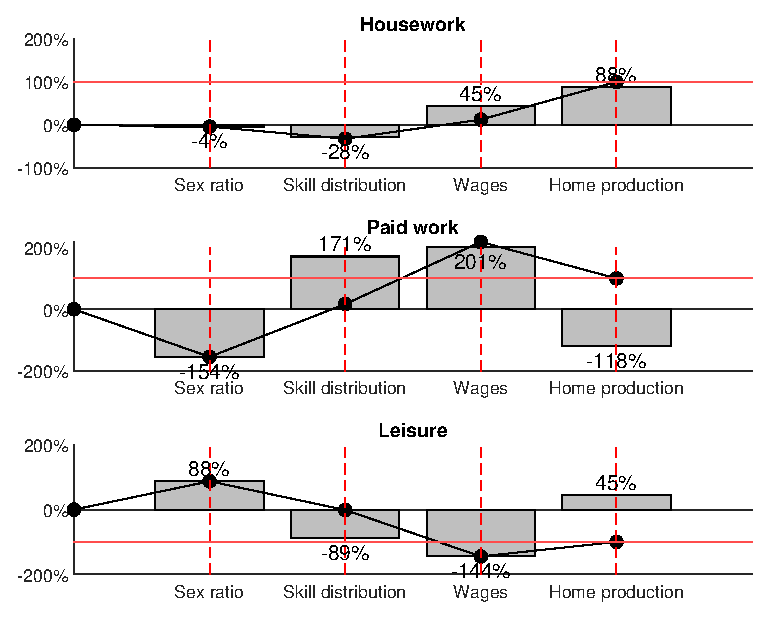
\includegraphics[width=.5\textwidth]{back_decomp_ta_m}}
	\note{The solid line with circle markers represents the cumulative change between 1990 and 2010, up to that factor. The bars represent the contribution of that factor alone to the total change. Forward decomposition starts at the 1990 steady state. Backward decomposition starts at the 2010 steady state.}
\end{figure}

\begin{figure}[hp]
	\centering
	\caption{Contributions to changes in assortative mating, 1990-2010}\label{fig:decomp_ms}
	\subfloat[Forward decomposition]{\includegraphics[width=.5\textwidth]{for_decomp_ms}}
	\\
	\subfloat[Backward decomposition]{\includegraphics[width=.5\textwidth]{back_decomp_ms}}
	\note{The solid line with circle markers represents the cumulative change between 1990 and 2010, up to that factor. The bars represent the contribution of that factor alone to the total change. Forward decomposition starts at the 1990 steady state. Backward decomposition starts at the 2010 steady state.}
\end{figure}

\subsubsection{The bargaining and marital sorting channels}

The sex ratio affects aggregate average resource allocation within the households via two channels. The first one is by improving wives outside option, which means that they enjoy a stronger bargaining position. The second one is thorugh changes in marital sorting, as the composition of households that are formed changes. If the effect of the sex ratios operates mainly through the second channel, actually a model with a unitary household would be a good representation of the way Chinese households allocate resources. 

Here I attempt to distinguish the effect of the two channels. The strategy I use goes as follows: in the backward and forward decompositions, I obtain the time allocation using the Pareto weights for each type of household in steady state after the sex ratio changes, but the marital sorting before it does. Then I compute what is the fraction of the total contribution of the sex ratio that is attributable to the changes in Pareto weights alone. This provides a measure of the contribution of the bargaining channel. I can do it the other way around, of course. That is, obtain the time allocation using the Pareto weights for each household in steady state before changing the sex ratio, and the marital sorting after it changes. This is the same issue that arises in the decomposition above in terms of the order of factors, except that now there are only two possible decompositions since there are only two changing factors.

I present the results of the exercise in table \ref{tab:sexratio_decomp}. I show here the two potential orderings for both the forward and backward decompositions. The message is clear: the bargaining channel plays a crucial role within the model in generating the effect of the sex ratio on married household time allocation. For any given of the three alternative uses of time, the fraction of the total effect of the sex ratio that is attributable to changes in Pareto weights and hence to bargaining is never lower than 44\% and in most cases is close to 100\%.

\begin{table}[htbp]
	\centering
	\caption{Decomposition of the effect of the sex ratio on time allocation for married people}
	\begin{tabular}{lrrrrr}
		\toprule
		\multicolumn{6}{c}{Forward decomposition} \\
		\midrule
		\multirow{2}[4]{*}{Statistic} & \multicolumn{2}{c}{$\Delta$Pareto weights} &       & \multicolumn{2}{c}{$\Delta$Marital sorting} \\
		\cmidrule{2-3}\cmidrule{5-6}      & \multicolumn{1}{l}{Bargaining} & \multicolumn{1}{l}{Sorting} &       & \multicolumn{1}{l}{Sorting} & \multicolumn{1}{l}{Bargaining} \\
		\midrule
		Married women housework & -44.10\% & -55.90\% &       & -52.25\% & -47.75\% \\
		Married women paid work & -105.15\% & 5.15\% &       & 4.36\% & -104.36\% \\
		Married women leisure & 104.27\% & -4.27\% &       & -4.57\% & 104.57\% \\
		Married men housework & -96.98\% & 196.98\% &       & 202.55\% & -102.55\% \\
		Married men paid work & 104.35\% & -4.35\% &       & -4.75\% & 104.75\% \\
		Married men leisure & -104.54\% & 4.54\% &       & 4.21\% & -104.21\% \\
		\midrule
		\multicolumn{6}{c}{Backward decomposition} \\
		\midrule
		\multirow{2}[4]{*}{Statistic} & \multicolumn{2}{c}{$\Delta$Pareto weights} &       & \multicolumn{2}{c}{$\Delta$Marital sorting} \\
		\cmidrule{2-3}\cmidrule{5-6}      & \multicolumn{1}{l}{Bargaining} & \multicolumn{1}{l}{Sorting} &       & \multicolumn{1}{l}{Sorting} & \multicolumn{1}{l}{Bargaining} \\
		\midrule
		Married women housework & 82.66\% & 17.34\% &       & 13.72\% & 86.28\% \\
		Married women paid work & 107.78\% & -7.78\% &       & -8.01\% & 108.01\% \\
		Married women leisure & -107.28\% & 7.28\% &       & 6.48\% & -106.48\% \\
		Married men housework & -95.65\% & -4.35\% &       & 0.47\% & -100.47\% \\
		Married men paid work & -105.71\% & 5.71\% &       & 5.23\% & -105.23\% \\
		Married men leisure & 105.26\% & -5.26\% &       & -5.48\% & 105.48\% \\
		\bottomrule
		\bottomrule
	\end{tabular}
	\label{tab:sexratio_decomp}
\end{table}

\subsection{The future increase in the sex ratio}

What should we expect to happen to marriage and household resource allocation as the sex ratio increases further? As I discussed in previous sections, the sex ratio among people of marriageable age may reach 1.2 men per woman around 2020. How big of an additional impact will this have for Chinese people? To answer this question, I compute a steady state with all the fundamental values of 2010, but with a sex ratio of 1.2 ($\theta_0=1.2$). The results are presented in table \ref{tab:quant_exp_1}.

\begin{table}[htbp]
	\centering
	\caption{The effects of a sex ratio of 1.2 in 2010}
	\begin{tabular}{lrrr}
		\toprule
		Statistic & \multicolumn{1}{l}{Baseline 2010} & \multicolumn{1}{l}{$\theta_0=1.2$} & \multicolumn{1}{l}{\% change} \\
		\midrule
		&       &       &  \\
		Married women housework & 15.06 & 14.97 & -0.54\% \\
		Married women paid work & 31.59 & 28.90 & -8.90\% \\
		Married women leisure & 71.36 & 74.13 & 3.81\% \\
		Married men housework & 2.56  & 2.58  & 0.91\% \\
		Married men paid work & 45.42 & 47.81 & 5.12\% \\
		Married men leisure & 70.02 & 67.61 & -3.50\% \\
		Single women housework & 5.54  & 5.54  & 0.00\% \\
		Single women paid work & 43.31 & 43.31 & 0.00\% \\
		Single women leisure & 69.15 & 69.15 & 0.00\% \\
		Single men housework & 1.23  & 1.23  & 0.00\% \\
		Single men paid work & 41.68 & 41.68 & 0.00\% \\
		Single men leisure & 75.09 & 75.09 & 0.00\% \\
		&       &       &  \\
		Married women consumption & 0.83  & 0.87  & 4.65\% \\
		Married men consumption & 1.08  & 1.05  & -3.14\% \\
		&       &       &  \\
		Average wife Pareto weight & 0.44  & 0.46  & 5.35\% \\
		&       &       &  \\
		Assortative mating measure & 1.52  & 1.55  & 2.15\% \\
		\bottomrule
		\bottomrule
	\end{tabular}
		\label{tab:quant_exp_1}
	\end{table}

The model predicts that in a steady state with a sex ratio of 1.2 in 2010, paid hours for married women are almost 9\% lower and 5\% higher for men. This is between one third and one half of the percent change between the 1990 and 2010 model steady states in both married female and male paid hours. Moreover, leisure time increases for women and decreases for men, about three and a half percentage points each. Assortative mating goes up very slightly. Finally, consumption for married women increases 4.65\% at the expense of a reduction of married men consumption of 3.14\%. An increase in the sex ratio has no effect on single people's time allocation, by construction of the model. Incorporating savings decisions would activate a channel by which the sex ratio would affect singles.

\subsection{The role of the gender wage gap}

In all previous exercises, I assume that the wages of men rose more than the wages of women between 1990 and 2010, as found by \cite{getao14}. This means that the gender wage gap increased between 1990 and 2010. As I discussed in section \ref{sec:dataandfacts}, this result may include composition effects, which are not relevant in this setting. The gender gap that is relevant in this study is on potential hourly earnings. In fact, I get a constant conditional gender wage gap with the CHNS data, albeit closer to the lower value in 2010. Therefore, I compute the steady state equilibrium in 2010 using the 1990 gender wage gap in order to assess how this changes results. In particular, I want to know if a constant gender wage gap helps the model perform better in relation to the data in 2010.

I present the result of this exercise in table \ref{tab:quant_exp_2}. A constant gender wage gap does bring the steady state time allocation a bit closer to the data, but only for married women. Notably, the leisure time for married people remains almost unchanged, as the lower gender wage gap with respect to the baseline mainly generates a reallocation of housework and paid work between wives and husbands. The fit of the model becomes a little bit worse for single females. Altogether, I conclude that a constant gender wage gap does not dramatically improve the model fit to the data in 2010. 

\begin{table}[]
	\centering
	\caption{The model in 2010 with a constant gender wage gap}
	\begin{tabular}{lccc}
		\toprule
		Statistic & \multicolumn{1}{p{4.045em}}{Data 2010} & \multicolumn{1}{p{6.455em}}{Baseline model 2010} & \multicolumn{1}{p{7.635em}}{Constant gender wage gap 2010} \\
		\midrule
		&       &       &  \\
		Married women housework & 11.27 & 15.06 & 13.87 \\
		Married women paid work & 35.87 & 31.59 & 32.59 \\
		Married women leisure & 70.86 & 71.36 & 71.54 \\
		Married men housework & 2.70  & 2.56  & 3.15 \\
		Married men paid work & 47.51 & 45.42 & 44.60 \\
		Married men leisure & 67.79 & 70.02 & 70.25 \\
		Single women housework & 4.50  & 5.54  & 5.58 \\
		Single women paid work & 45.06 & 43.31 & 42.75 \\
		Single women leisure & 68.44 & 69.15 & 69.67 \\
		Single men housework & 1.59  & 1.23  & 1.23 \\
		Single men paid work & 42.73 & 41.68 & 41.68 \\
		Single men leisure & 73.69 & 75.09 & 75.09 \\
		&       &       &  \\
		Married women consumption &       & 0.83  & 0.90 \\
		Married men consumption &       & 1.08  & 1.08 \\
		&       &       &  \\
		Average wife Pareto weight &       & 0.44  & 0.46 \\
		&       &       &  \\
		Assortative mating measure & 1.63  & 1.52  & 1.52 \\
		\bottomrule
		\bottomrule
	\end{tabular}
	\label{tab:quant_exp_2}
\end{table}

Finally, I go a step further and ask what would happen if there were no gender wage gap at all. The previous exercise hints at the direction of the changes, but to properly answer the question I present the results for the steady state in 2010 with no gender wage gap next to the results for the baseline model in 2010 in table \ref{tab:quant_exp_3}.

Not surprisingly, the removal of the sex ratio leads to housework time becoming more equal across husband and wives, although a gap of about seven hours per week persists. This is a result of the weight of female housework time being larger than one half ($\eta_f=0.58$) in the housework time aggregator for married couples. And again, leisure time remains largely unchanged for both females and males. 

Married women consumption goes up substantially. Interestingly married men consumption also increases slightly. As both leisure and consumption rise for the latter, it seems that a reduction of the gender wage gap benefits both men and women in the model. This is less trivial than it appears at first. The drop in the gender wage gap affects time allocation via two channels: subsitution of husband for wife paid work, and an increase in the bargaining position of females as the value of their outside option increases, as reflected by the larger Pareto weight in the steady state with no gender wage gap. These two channels operate in opposite directions, and therefore ex ante is uncertain which one will prevail. It seems therefore that policies that attempt to reduce the gender wage gap would be beneficial for married people in general.  

\begin{table}[]
	\centering
	\caption{The model in 2010 with no gender wage gap}
	\begin{tabular}{lrrr}
		\toprule
		Statistic & \multicolumn{1}{l}{Baseline 2010} & \multicolumn{1}{l}{No gender wage gap} & \multicolumn{1}{l}{\% change} \\
		\midrule
		&       &       &  \\
		Married women housework & 15.06 & 11.82 & -24.17\% \\
		Married women paid work & 31.59 & 34.37 & 8.45\% \\
		Married women leisure & 71.36 & 71.80 & 0.63\% \\
		Married men housework & 2.56  & 4.50  & 56.41\% \\
		Married men paid work & 45.42 & 42.81 & -5.91\% \\
		Married men leisure & 70.02 & 70.68 & 0.95\% \\
		Single women housework & 5.54  & 5.64  & 1.77\% \\
		Single women paid work & 43.31 & 41.77 & -3.61\% \\
		Single women leisure & 69.15 & 70.59 & 2.06\% \\
		Single men housework & 1.23  & 1.23  & 0.00\% \\
		Single men paid work & 41.68 & 41.68 & 0.00\% \\
		Single men leisure & 75.09 & 75.09 & 0.00\% \\
		&       &       &  \\
		Married women consumption & 0.83  & 1.04  & 22.51\% \\
		Married men consumption & 1.08  & 1.09  & 1.12\% \\
		&       &       &  \\
		Average wife Pareto weight & 0.44  & 0.50  & 14.10\% \\
		&       &       &  \\
		Assortative mating measure & 1.52  & 1.52  & 0.16\% \\
		\bottomrule
		\bottomrule
	\end{tabular}
	\label{tab:quant_exp_3}
\end{table}


\section{Conclusions} \label{sec:conclusions}

This paper explores the effect changes in the sex ratio has on marital sorting, bargaining and time allocation between spouses. It does so by building a model of marriage that allows for people with different education levels to marry. Moreover, it allows for bargaining over its gains to affect the amount of paid work, housework and leisure each spouse does or enjoys. 

The model is calibrated to reproduce time allocation and marital sorting data for China in 1990. It does so successfully. A set of quantitative exercises are subsequently performed.

I find that the sex ratio accounts for between one third and one half of the changes in paid work and leisure time for married women between 1990 and 2010. Moreover, most of the change operates via bargaining and very little via marital sorting. I run a counterfactual exercise and find that had the sex ratio reached 1.2 men per woman in 2010, paid hours would have been almost 9\% lower for married females and 5\% higher for their male counterparts. Eliminating the gender wage gap would have a similar impact on women, but would decrease men's paid work hours by 6\%.

A number of extensions or improvements could be made to the present work. The most obvious would be to endogeneize the education decision. Agents could face a tradeoff in a pre-marriage-market period between acquiring more education and exerting effort. Second, adding savings decisions would create interactions between he sex ratio and single people's time allocation that are not present in the model, albeit it would considerably increase the difficulty of defining, computing the equilibrium and calibrating the model. Finally, being able to make finer refinements (geographically, in terms of skills) could improve our knowledge of time allocation patterns across different types of households and allow for better testing of the rich dynamics in the model.  

%I find that had the sex ratio stayed at its 1990 level, married females would have worked roughly 30\% more hours per week outside the house, while assortative mating would've been only slightly lower. A further increase in the sex ratio to 1.2 men per woman would decrease the paid work hours of married women to 22 per week, around half of the hours worked in 1990, and increased very slightly the levels of assortive mating. Finally, an increase in the wage of women relative to men from 0.75 to 0.85 would increase hours worked for women by only 20\%, leaving them still way below their 1990 level.
%
%An analysis of changes in the Pareto weights reveals that the increase in the sex ratio benefits all women, but not equally. Complex interactions between the sex ratios among people with different education levels and the wage gains between 1990 and 2010 produce the largest gain for women with primary education completed. The two extremes of the distribution, women with no schooling and those with college and more, experience opposite forces affecting their bargaining position over marriage gains. While the sex ratio among people with no education fell while they lagged behing in wages, the opposite happened for college educated people. The effect of the changes in wages seemed in both cases to dominate the effect of changes in the sex ratio, increasing the share of resources in marriage that women take for the college educated and decreasing it for the ones with no schooling. 

\singlespacing
\bibliographystyle{plainnat}
\bibliography{bibliography}

\clearpage

\onehalfspacing

%\section*{Tables} \label{sec:tab}
%\addcontentsline{toc}{section}{Tables}

%\begin{table}[htbp]
%	\centering
%	\caption{Sex ratio at birth (male births over female births), 1982-2010}
%	\begin{tabular}{lr}
%		\toprule
%		Year & \multicolumn{1}{l}{Sex ratio at birth} \\
%		\midrule
%		1982 & 1.085 \\
%		1990 & 1.113 \\
%		2000 & 1.169 \\
%		2010 & 1.179 \\
%		\bottomrule
%	\end{tabular}
%	\label{srb_census}
%	\source{Tabulation on the Population Census of the People's Republic of China, National Bureau of Statistics}
%\end{table}

%\begin{table}[htbp]
%	\centering
%	\caption{Contingency table: assortative mating in 1990}
%	\begin{tabular}{lrrrrrrrrrr}
%		\toprule
%		\multicolumn{1}{c}{\multirow{2}[1]{*}{Wife}} & \multicolumn{10}{c}{Husband} \\
%		& \multicolumn{2}{c}{NS} & \multicolumn{2}{c}{P} & \multicolumn{2}{c}{LM} & \multicolumn{2}{c}{UM} & \multicolumn{2}{c}{C} \\
%		NS & \textbf{0.073} & \textbf{0.030} & 0.087 & 0.063 & 0.090 & 0.120 & 0.032 & 0.059 & 0.002 & 0.013 \\
%		P & 0.017 & 0.023 & \textbf{0.073} & \textbf{0.048} & 0.090 & 0.092 & 0.034 & 0.045 & 0.004 & 0.010 \\
%		LM & 0.012 & 0.033 & 0.045 & 0.069 & \textbf{0.174} & \textbf{0.132} & 0.074 & 0.065 & 0.009 & 0.014 \\
%		UM & 0.004 & 0.016 & 0.013 & 0.034 & 0.062 & 0.065 & \textbf{0.061} & \textbf{0.032} & 0.014 & 0.007 \\
%		C & 0.000 & 0.003 & 0.001 & 0.006 & 0.003 & 0.012 & 0.008 & 0.006 & \textbf{0.017} & \textbf{0.001} \\
%		\bottomrule
%	\end{tabular}
%	\label{cont_tab_1990}
%	\source{Author's calculations using the China Health and Nutrition Survey}
%\end{table}
%
%\begin{table}[htbp]
%	\centering
%	\caption{Distribution of education and wages}\label{education}
%	\begin{tabular}{lrrrrr}
%		\toprule
%		\multicolumn{1}{c}{\multirow{2}[4]{*}{Education}} & \multicolumn{2}{c}{1990} &   & \multicolumn{2}{c}{2010} \\
%		\cmidrule{2-3}\cmidrule{5-6}      & \multicolumn{1}{l}{Female} & \multicolumn{1}{l}{Male} &   & \multicolumn{1}{l}{Female} & \multicolumn{1}{l}{Male} \\
%		\midrule
%		\multicolumn{6}{c}{Distribution} \\
%		\midrule
%		NS & 0,2554 & 0,1089 &   & 0,0510 & 0,0302 \\
%		P & 0,2134 & 0,2192 &   & 0,1267 & 0,1063 \\
%		LM & 0,3399 & 0,4310 &   & 0,4008 & 0,4239 \\
%		UM & 0,1545 & 0,1962 &   & 0,1116 & 0,1546 \\
%		C+ & 0,0369 & 0,0447 &   & 0,3099 & 0,2850 \\
%		\midrule
%		\multicolumn{6}{c}{Wages} \\
%		\midrule
%		NS & 0,7284 & 1,0000 &   & 3,2149 & 3,7822 \\
%		P & 0,7284 & 1,0000 &   & 4,1027 & 4,8267 \\
%		LM & 0,7284 & 1,0000 &   & 4,7647 & 5,6055 \\
%		UM & 0,7284 & 1,0000 &   & 4,9104 & 5,7770 \\
%		C+ & 0,7284 & 1,0000 &   & 7,6939 & 9,0517 \\
%		\bottomrule
%	\end{tabular}
%\end{table}

%\begin{table}
%	\centering
%	\caption{Parameters not calibrated}\label{param_not_calib}
%	\begin{tabular}{lrr}
%		\toprule
%		\multicolumn{3}{c}{Externally chosen parameters} \\
%		\midrule
%		Parameter & \multicolumn{1}{l}{Value} & \multicolumn{1}{l}{Source} \\
%		\midrule
%		$\beta$ & 0,9600 & \multicolumn{1}{l}{Standard} \\
%		$\sigma$ & 1,5000 & \multicolumn{1}{l}{Attanasio et al. (2008)} \\
%		$\delta$ & 0,0203 & \multicolumn{1}{l}{Inverse of life expectancy at 20 years} \\
%		$\alpha_g$ & 0,9500 & \multicolumn{1}{l}{Share of home equipment over total consumption expenditure} \\
%		$A_g$ (1990) & 1,0000 & \multicolumn{1}{l}{Normalization} \\
%		$A_g$ (2010) & 3,7822 & \multicolumn{1}{l}{Productivity growth since 1990} \\
%		\midrule
%		\multicolumn{3}{c}{Parameters chosen to exactly match data} \\
%		\midrule
%		Parameter & \multicolumn{1}{l}{Value} & \multicolumn{1}{l}{Set to match} \\
%		\midrule
%		$\eta$ & 0,3072 & \multicolumn{1}{l}{Change in husband to wife housework ratio between 1990 and 2010} \\
%		$\eta_f$ & 0,5384 & \multicolumn{1}{l}{Level of husband to wife housework ratio in 1990} \\
%		\multicolumn{2}{c}{Single women} &  \\
%		$\sigma_c$  & 0,3526 &  \\
%		$\sigma_l$  & 0,6229 & \multicolumn{1}{l}{Single women time allocation} \\
%		$\sigma_g$ & 0,0245 &  \\
%		\multicolumn{2}{c}{Single men} &  \\
%		$\sigma_c$  & 0,3635 &  \\
%		$\sigma_l$  & 0,6342 & \multicolumn{1}{l}{Single men time allocation} \\
%		$\sigma_g$ & 0,0023 &  \\
%		\bottomrule
%	\end{tabular}
%\end{table}

%\begin{table}
%	\centering
%	\caption{Calibrated parameters}\label{param_calib}
%	\begin{tabular}{lrl}
%		\toprule
%		Parameter & \multicolumn{1}{l}{Value} & Target \\
%		\midrule
%		\multicolumn{2}{c}{Married agents} &  \\
%		$\sigma_c$  & 0,3450 &  \\
%		$\sigma_l$  & 0,6150 & Married households time allocation \\
%		$\sigma_g$ & 0,0400 &  \\
%		&   &  \\
%		$\mu_{z_f,z_m}$ & \multicolumn{1}{l}{25 different values} & Marital sorting \\
%		&   &  \\
%		$\psi_f$ & -1,0000 & Husband to wife leisure ratio \\
%		\bottomrule
%	\end{tabular}
%\end{table}
%
%	\begin{table}[htbp]
%	\centering
%	\caption{Time allocation results (hours per week)}\label{ta_results}
%	\begin{tabular}{lrrrrr}
%		\toprule
%		\multicolumn{1}{c}{\multirow{2}[4]{*}{Statistic}} & \multicolumn{2}{c}{1990} &   & \multicolumn{2}{c}{2010} \\
%		\cmidrule{2-3}\cmidrule{5-6}      & \multicolumn{1}{l}{Data} & \multicolumn{1}{l}{Model} &   & \multicolumn{1}{l}{Data} & \multicolumn{1}{l}{Model} \\
%		\midrule
%		Wives housework time & 18,09 & 18,57 &   & 11,27 & 12,48 \\
%		Wives paid work time & 41,10 & 41,15 &   & 35,87 & 27,27 \\
%		Wives leisure time & 58,82 & 58,28 &   & 70,86 & 78,26 \\
%		Husbands housework time & 3,91 & 4,01 &   & 2,70 & 3,49 \\
%		Husbands paid work time & 47,38 & 47,96 &   & 47,51 & 54,03 \\
%		Husbands leisure time & 66,71 & 66,03 &   & 67,79 & 60,49 \\
%		&   &   &   &   &  \\
%		Single women housework time & 7,39 & 7,39 &   & 4,50 & 4,27 \\
%		Single women paid work time & 48,00 & 48,00 &   & 45,06 & 44,36 \\
%		Single women leisure time & 62,61 & 62,61 &   & 68,44 & 69,37 \\
%		Single men housework time & 1,66 & 1,66 &   & 1,59 & 0,93 \\
%		Single men paid work time & 47,55 & 47,55 &   & 42,73 & 43,15 \\
%		Single men leisure time & 68,79 & 68,78 &   & 73,69 & 73,92 \\
%		\bottomrule
%	\end{tabular}
%\end{table}
%
%	\begin{table}[htbp]
%	\centering
%	\caption{Marital sorting results 1990}\label{mar_sort_1990}
%	\begin{tabular}{lccccccccccr}
%		\toprule
%		\multicolumn{12}{c}{Data} \\
%		\midrule
%		\multicolumn{1}{c}{\multirow{2}[3]{*}{Wife}} & \multicolumn{10}{c}{Husband}          &  \\
%		\cmidrule{2-11}  & \multicolumn{2}{c}{NS} & \multicolumn{2}{c}{P} & \multicolumn{2}{c}{LM} & \multicolumn{2}{c}{UM} & \multicolumn{2}{c}{C+} & \multicolumn{1}{l}{Marginal} \\
%		NS & \multicolumn{1}{r}{\textcolor[rgb]{ 1,  0,  0}{0,073}} & \multicolumn{1}{r}{\textcolor[rgb]{ .122,  .306,  .471}{0,026}} & \multicolumn{1}{r}{0,087} & \multicolumn{1}{r}{0,062} & \multicolumn{1}{r}{0,090} & \multicolumn{1}{r}{0,124} & \multicolumn{1}{r}{0,032} & \multicolumn{1}{r}{0,060} & \multicolumn{1}{r}{0,002} & \multicolumn{1}{r}{0,015} & 0,286 \\
%		P & \multicolumn{1}{r}{0,017} & \multicolumn{1}{r}{0,020} & \multicolumn{1}{r}{\textcolor[rgb]{ 1,  0,  0}{0,073}} & \multicolumn{1}{r}{\textcolor[rgb]{ .122,  .306,  .471}{0,047}} & \multicolumn{1}{r}{0,090} & \multicolumn{1}{r}{0,094} & \multicolumn{1}{r}{0,034} & \multicolumn{1}{r}{0,046} & \multicolumn{1}{r}{0,004} & \multicolumn{1}{r}{0,011} & 0,218 \\
%		LM & \multicolumn{1}{r}{0,012} & \multicolumn{1}{r}{0,028} & \multicolumn{1}{r}{0,045} & \multicolumn{1}{r}{0,068} & \multicolumn{1}{r}{\textcolor[rgb]{ 1,  0,  0}{0,174}} & \multicolumn{1}{r}{\textcolor[rgb]{ .122,  .306,  .471}{0,136}} & \multicolumn{1}{r}{0,074} & \multicolumn{1}{r}{0,066} & \multicolumn{1}{r}{0,009} & \multicolumn{1}{r}{0,016} & 0,314 \\
%		UM & \multicolumn{1}{r}{0,004} & \multicolumn{1}{r}{0,014} & \multicolumn{1}{r}{0,013} & \multicolumn{1}{r}{0,033} & \multicolumn{1}{r}{0,062} & \multicolumn{1}{r}{0,067} & \multicolumn{1}{r}{\textcolor[rgb]{ 1,  0,  0}{0,061}} & \multicolumn{1}{r}{\textcolor[rgb]{ .122,  .306,  .471}{0,032}} & \multicolumn{1}{r}{0,014} & \multicolumn{1}{r}{0,008} & 0,154 \\
%		C+ & \multicolumn{1}{r}{0,000} & \multicolumn{1}{r}{0,003} & \multicolumn{1}{r}{0,001} & \multicolumn{1}{r}{0,006} & \multicolumn{1}{r}{0,003} & \multicolumn{1}{r}{0,012} & \multicolumn{1}{r}{0,008} & \multicolumn{1}{r}{0,006} & \multicolumn{1}{r}{\textcolor[rgb]{ 1,  0,  0}{0,017}} & \multicolumn{1}{r}{\textcolor[rgb]{ .122,  .306,  .471}{0,001}} & 0,028 \\
%		Marginal & \multicolumn{2}{c}{0,107} & \multicolumn{2}{c}{0,219} & \multicolumn{2}{c}{0,421} & \multicolumn{2}{c}{0,208} & \multicolumn{2}{c}{0,046} &  \\
%		\midrule
%		\multicolumn{12}{c}{Model} \\
%		\midrule
%		NS & \multicolumn{1}{r}{\textcolor[rgb]{ 1,  0,  0}{0,043}} & \multicolumn{1}{r}{\textcolor[rgb]{ .122,  .306,  .471}{0,024}} & \multicolumn{1}{r}{0,087} & \multicolumn{1}{r}{0,057} & \multicolumn{1}{r}{0,090} & \multicolumn{1}{r}{0,113} & \multicolumn{1}{r}{0,035} & \multicolumn{1}{r}{0,054} & \multicolumn{1}{r}{0,006} & \multicolumn{1}{r}{0,014} & 0,261 \\
%		P & \multicolumn{1}{r}{0,020} & \multicolumn{1}{r}{0,019} & \multicolumn{1}{r}{\textcolor[rgb]{ 1,  0,  0}{0,062}} & \multicolumn{1}{r}{\textcolor[rgb]{ .122,  .306,  .471}{0,047}} & \multicolumn{1}{r}{0,090} & \multicolumn{1}{r}{0,093} & \multicolumn{1}{r}{0,036} & \multicolumn{1}{r}{0,045} & \multicolumn{1}{r}{0,008} & \multicolumn{1}{r}{0,011} & 0,215 \\
%		LM & \multicolumn{1}{r}{0,015} & \multicolumn{1}{r}{0,030} & \multicolumn{1}{r}{0,047} & \multicolumn{1}{r}{0,072} & \multicolumn{1}{r}{\textcolor[rgb]{ 1,  0,  0}{0,183}} & \multicolumn{1}{r}{\textcolor[rgb]{ .122,  .306,  .471}{0,143}} & \multicolumn{1}{r}{0,074} & \multicolumn{1}{r}{0,069} & \multicolumn{1}{r}{0,013} & \multicolumn{1}{r}{0,017} & 0,332 \\
%		UM & \multicolumn{1}{r}{0,008} & \multicolumn{1}{r}{0,014} & \multicolumn{1}{r}{0,016} & \multicolumn{1}{r}{0,034} & \multicolumn{1}{r}{0,063} & \multicolumn{1}{r}{0,068} & \multicolumn{1}{r}{\textcolor[rgb]{ 1,  0,  0}{0,053}} & \multicolumn{1}{r}{\textcolor[rgb]{ .122,  .306,  .471}{0,033}} & \multicolumn{1}{r}{0,017} & \multicolumn{1}{r}{0,008} & 0,157 \\
%		C+ & \multicolumn{1}{r}{0,004} & \multicolumn{1}{r}{0,003} & \multicolumn{1}{r}{0,005} & \multicolumn{1}{r}{0,008} & \multicolumn{1}{r}{0,007} & \multicolumn{1}{r}{0,015} & \multicolumn{1}{r}{0,011} & \multicolumn{1}{r}{0,007} & \multicolumn{1}{r}{\textcolor[rgb]{ 1,  0,  0}{0,008}} & \multicolumn{1}{r}{\textcolor[rgb]{ .122,  .306,  .471}{0,002}} & 0,035 \\
%		Marginal & \multicolumn{2}{c}{0,090} & \multicolumn{2}{c}{0,217} & \multicolumn{2}{c}{0,432} & \multicolumn{2}{c}{0,209} & \multicolumn{2}{c}{0,052} &  \\
%		\bottomrule
%	\end{tabular}
%\end{table}
%
%	\begin{table}[htbp]
%	\centering
%	\caption{Marital sorting results 2010}\label{mar_sort_2010}
%	\begin{tabular}{lccccccccccr}
%		\toprule
%		\multicolumn{12}{c}{Data} \\
%		\midrule
%		\multicolumn{1}{c}{\multirow{2}[3]{*}{Wife}} & \multicolumn{10}{c}{Husband}          &  \\
%		\cmidrule{2-11}      & \multicolumn{2}{c}{NS} & \multicolumn{2}{c}{P} & \multicolumn{2}{c}{LM} & \multicolumn{2}{c}{UM} & \multicolumn{2}{c}{C+} & \multicolumn{1}{l}{Marginal} \\
%		NS & \multicolumn{1}{r}{\textcolor[rgb]{ 1,  0,  0}{0,017}} & \multicolumn{1}{r}{\textcolor[rgb]{ .122,  .306,  .471}{0,002}} & \multicolumn{1}{r}{0,013} & \multicolumn{1}{r}{0,006} & \multicolumn{1}{r}{0,023} & \multicolumn{1}{r}{0,026} & \multicolumn{1}{r}{0,002} & \multicolumn{1}{r}{0,008} & \multicolumn{1}{r}{0,000} & \multicolumn{1}{r}{0,013} & 0,055 \\
%		P & \multicolumn{1}{r}{0,010} & \multicolumn{1}{r}{0,005} & \multicolumn{1}{r}{\textcolor[rgb]{ 1,  0,  0}{0,060}} & \multicolumn{1}{r}{\textcolor[rgb]{ .122,  .306,  .471}{0,018}} & \multicolumn{1}{r}{0,068} & \multicolumn{1}{r}{0,069} & \multicolumn{1}{r}{0,008} & \multicolumn{1}{r}{0,021} & \multicolumn{1}{r}{0,002} & \multicolumn{1}{r}{0,034} & 0,147 \\
%		LM & \multicolumn{1}{r}{0,008} & \multicolumn{1}{r}{0,016} & \multicolumn{1}{r}{0,035} & \multicolumn{1}{r}{0,052} & \multicolumn{1}{r}{\textcolor[rgb]{ 1,  0,  0}{0,291}} & \multicolumn{1}{r}{\textcolor[rgb]{ .122,  .306,  .471}{0,206}} & \multicolumn{1}{r}{0,060} & \multicolumn{1}{r}{0,062} & \multicolumn{1}{r}{0,043} & \multicolumn{1}{r}{0,101} & 0,436 \\
%		UM & \multicolumn{1}{r}{0,002} & \multicolumn{1}{r}{0,004} & \multicolumn{1}{r}{0,007} & \multicolumn{1}{r}{0,014} & \multicolumn{1}{r}{0,041} & \multicolumn{1}{r}{0,055} & \multicolumn{1}{r}{\textcolor[rgb]{ 1,  0,  0}{0,041}} & \multicolumn{1}{r}{\textcolor[rgb]{ .122,  .306,  .471}{0,016}} & \multicolumn{1}{r}{0,025} & \multicolumn{1}{r}{0,027} & 0,116 \\
%		C+ & \multicolumn{1}{r}{0,000} & \multicolumn{1}{r}{0,009} & \multicolumn{1}{r}{0,005} & \multicolumn{1}{r}{0,029} & \multicolumn{1}{r}{0,048} & \multicolumn{1}{r}{0,116} & \multicolumn{1}{r}{0,031} & \multicolumn{1}{r}{0,035} & \multicolumn{1}{r}{\textcolor[rgb]{ 1,  0,  0}{0,162}} & \multicolumn{1}{r}{\textcolor[rgb]{ .122,  .306,  .471}{0,057}} & 0,246 \\
%		Marginal & \multicolumn{2}{c}{0,036} & \multicolumn{2}{c}{0,119} & \multicolumn{2}{c}{0,471} & \multicolumn{2}{c}{0,142} & \multicolumn{2}{c}{0,231} &  \\
%		\midrule
%		\multicolumn{12}{c}{Model} \\
%		\midrule
%		NS & \multicolumn{1}{r}{\textcolor[rgb]{ 1,  0,  0}{0,010}} & \multicolumn{1}{r}{\textcolor[rgb]{ .122,  .306,  .471}{0,001}} & \multicolumn{1}{r}{0,006} & \multicolumn{1}{r}{0,003} & \multicolumn{1}{r}{0,015} & \multicolumn{1}{r}{0,016} & \multicolumn{1}{r}{0,007} & \multicolumn{1}{r}{0,009} & \multicolumn{1}{r}{0,002} & \multicolumn{1}{r}{0,012} & 0,041 \\
%		P & \multicolumn{1}{r}{0,004} & \multicolumn{1}{r}{0,004} & \multicolumn{1}{r}{\textcolor[rgb]{ 1,  0,  0}{0,025}} & \multicolumn{1}{r}{\textcolor[rgb]{ .122,  .306,  .471}{0,010}} & \multicolumn{1}{r}{0,059} & \multicolumn{1}{r}{0,048} & \multicolumn{1}{r}{0,024} & \multicolumn{1}{r}{0,028} & \multicolumn{1}{r}{0,015} & \multicolumn{1}{r}{0,036} & 0,127 \\
%		LM & \multicolumn{1}{r}{0,006} & \multicolumn{1}{r}{0,013} & \multicolumn{1}{r}{0,022} & \multicolumn{1}{r}{0,028} & \multicolumn{1}{r}{\textcolor[rgb]{ 1,  0,  0}{0,210}} & \multicolumn{1}{r}{\textcolor[rgb]{ .122,  .306,  .471}{0,144}} & \multicolumn{1}{r}{0,081} & \multicolumn{1}{r}{0,084} & \multicolumn{1}{r}{0,057} & \multicolumn{1}{r}{0,108} & 0,377 \\
%		UM & \multicolumn{1}{r}{0,002} & \multicolumn{1}{r}{0,005} & \multicolumn{1}{r}{0,004} & \multicolumn{1}{r}{0,011} & \multicolumn{1}{r}{0,040} & \multicolumn{1}{r}{0,055} & \multicolumn{1}{r}{\textcolor[rgb]{ 1,  0,  0}{0,033}} & \multicolumn{1}{r}{\textcolor[rgb]{ .122,  .306,  .471}{0,032}} & \multicolumn{1}{r}{0,065} & \multicolumn{1}{r}{0,041} & 0,144 \\
%		C+ & \multicolumn{1}{r}{0,012} & \multicolumn{1}{r}{0,010} & \multicolumn{1}{r}{0,017} & \multicolumn{1}{r}{0,024} & \multicolumn{1}{r}{0,057} & \multicolumn{1}{r}{0,119} & \multicolumn{1}{r}{0,079} & \multicolumn{1}{r}{0,070} & \multicolumn{1}{r}{\textcolor[rgb]{ 1,  0,  0}{0,147}} & \multicolumn{1}{r}{\textcolor[rgb]{ .122,  .306,  .471}{0,089}} & 0,312 \\
%		Marginal & \multicolumn{2}{c}{0,034} & \multicolumn{2}{c}{0,076} & \multicolumn{2}{c}{0,382} & \multicolumn{2}{c}{0,223} & \multicolumn{2}{c}{0,286} & 1,000 \\
%		\bottomrule
%	\end{tabular}
%\end{table}
%
%\begin{table}
%	\centering
%	\caption{Simulation results}\label{sim_res}
%	\begin{tabular}{lrrrr}
%		\toprule
%		Statistic & \multicolumn{1}{l}{Model 2010} & \multicolumn{1}{l}{Sim 1} & \multicolumn{1}{l}{Sim 2} & \multicolumn{1}{l}{Sim 3} \\
%		\midrule
%		&   &   &   &  \\
%		Wives housework time & 12,48 & 10,23 & 10,82 & 9,61 \\
%		Wives paid work time & 27,27 & 35,85 & 21,96 & 24,20 \\
%		Wives leisure time & 78,26 & 71,92 & 85,23 & 84,19 \\
%		Husbands housework time & 3,49 & 3,13 & 2,83 & 3,62 \\
%		Husbands paid work time & 54,03 & 48,43 & 58,48 & 57,49 \\
%		Husbands leisure time & 60,49 & 66,46 & 56,69 & 56,89 \\
%		&   &   &   &  \\
%		Assortative mating measure & 1,54 & 1,52 & 1,55 & 1,55 \\
%		&   &   &   &  \\
%		Average Pareto weight wives & 0,52 & 0,47 & 0,57 & 0,59 \\
%		\bottomrule
%	\end{tabular}
%\end{table}
%
%\begin{table}
%	\centering
%	\caption{Average Pareto weight of women by education}\label{pweights}
%	\begin{tabular}{lrrrrr}
%		\toprule
%		Education & 1990 & 2010 & \multicolumn{1}{l}{Sim 1} & \multicolumn{1}{l}{Sim 2} & \multicolumn{1}{l}{Sim 3} \\
%		\midrule
%		NS & 0,126 & 0,095 & 0,084 & 0,108 & 0,119 \\
%		P & 0,374 & 0,315 & 0,211 & 0,404 & 0,435 \\
%		LM & 0,470 & 0,484 & 0,426 & 0,531 & 0,558 \\
%		UM & 0,608 & 0,558 & 0,517 & 0,604 & 0,623 \\
%		C+ & 0,679 & 0,696 & 0,629 & 0,752 & 0,769 \\
%		\bottomrule
%	\end{tabular}
%\end{table}

%\newpage
%
%\section*{Figures} \label{sec:fig}
%\addcontentsline{toc}{section}{Figures}

%\begin{figure}[hp]
%  \centering
%  \caption{Estimated and projected sex ratio at birth in China (1970-2070)}
%  \includegraphics[width=.6\textwidth]{srb_un}
%  \label{srb_1970_2070}
%  \source{United Nations Population Division}
%\end{figure}
%
%\begin{figure}[hp]
%	\centering
%	\caption{Projected sex ratio for different marriageable age ranges in China}
%	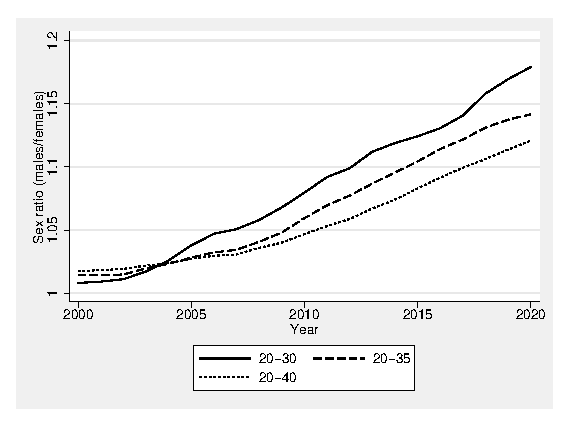
\includegraphics[width=.6\textwidth]{srma_2000census}
%	\label{srma_census}
%	\source{Chinese 2000 census}
%\end{figure}


%\begin{figure}[hp]
%	\centering
%	\caption{Labor force participation in China, people aged 20-40 not attending school (1990-2010)}\label{lfp}
%	\subfloat[Extensive margin]{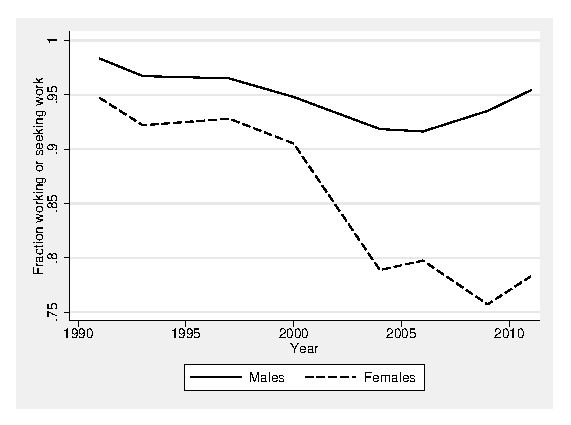
\includegraphics[width=.6\textwidth]{lfp_overall_sex}}
%	\\
%	\subfloat[Intensive margin]{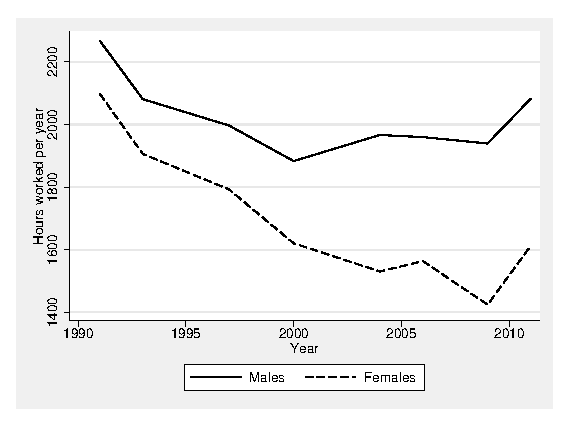
\includegraphics[width=.6\textwidth]{lfp_intensive_sex}}
%	\source{Author's calculations using the China Health and Nutrition Survey}
%\end{figure}
%
%\begin{figure}[hp]
%	\centering
%	\caption{Labor force participation in China by marital status, people aged 20-40 not attending school (1990-2010)}\label{lfp_marst}
%	\subfloat[Extensive margin]{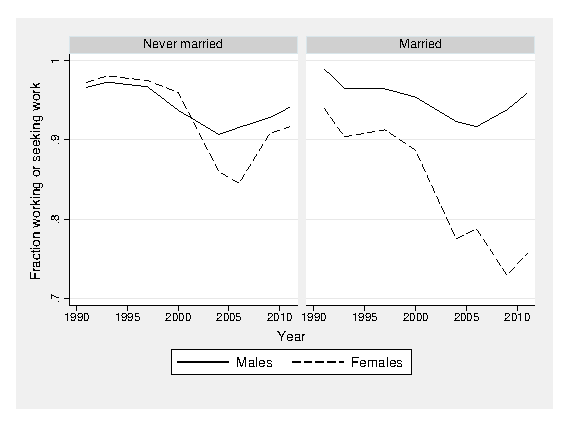
\includegraphics[width=.6\textwidth]{lfp_overall_sex_marst}}
%	\\
%	\subfloat[Intensive margin]{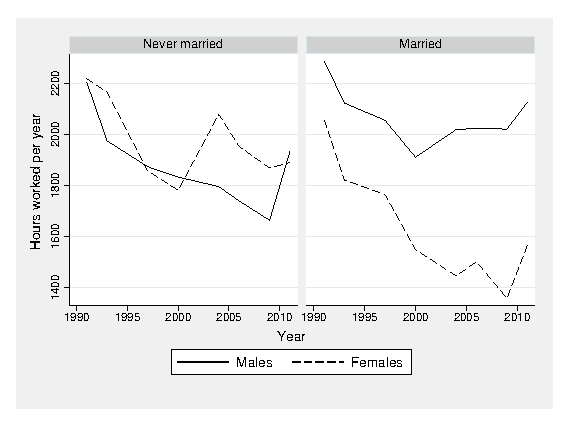
\includegraphics[width=.6\textwidth]{lfp_intensive_sex_marst}}
%	\source{Author's calculations using the China Health and Nutrition Survey}
%\end{figure}
%
%\begin{figure}
%	\centering
%	\caption{Time allocation of Chinese married people, 1990-2010}\label{time_use_married}
%	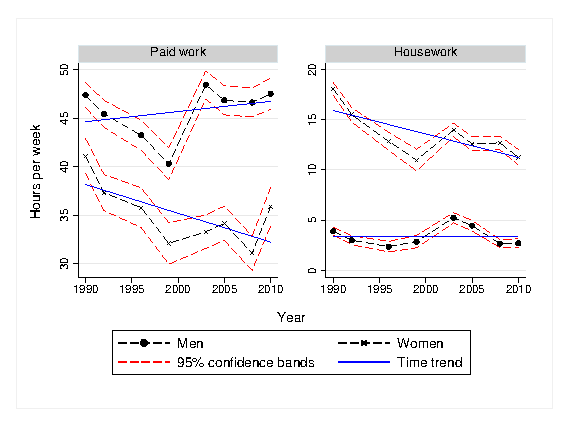
\includegraphics[width=.6\textwidth]{time_use_married}
%	\source{Author's calculations using the China Health and Nutrition Survey}
%\end{figure}
%
%\begin{figure}[hp]
%	\centering
%	\caption{Real hourly wages by sex in China, 1990-2010}
%	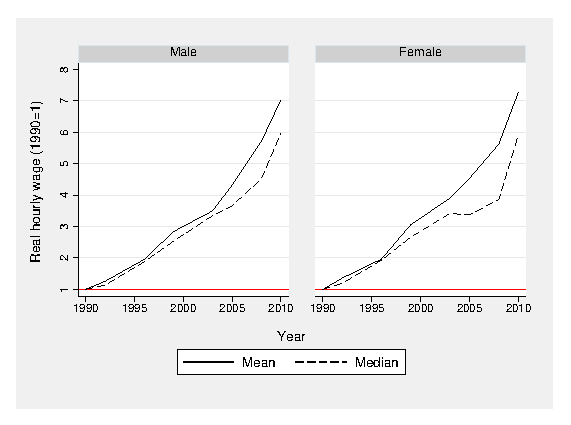
\includegraphics[width=.6\textwidth]{hourly_wages_1990_2010}
%	\label{real_hourly_wages_1990_2010}
%	\source{Author's calculations using the China Health and Nutrition Survey}
%\end{figure}
%
%\begin{figure}
%	\centering
%	\caption{Gender wage ratio in China, 1990-2010}\label{gender_wage_ratio}
%	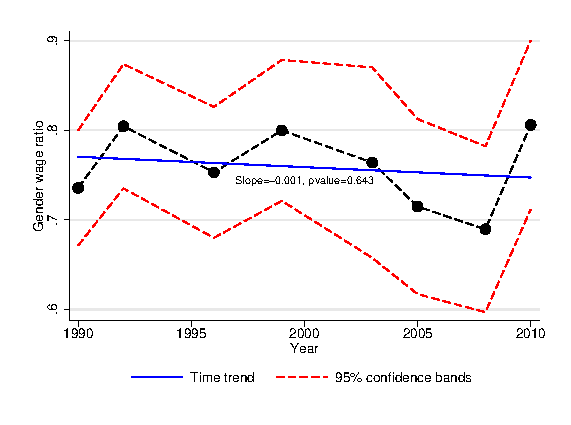
\includegraphics[width=.6\textwidth]{gender_wage_ratio}
%	\source{Author's calculations using the China Health and Nutrition Survey}
%\end{figure}
%
%
%
%
%
%\begin{figure}[hp]
%	\centering
%	\caption{Household income per capita inequality in China, 1990-2010}\label{hhincpc_cpi_gini}
%	\includegraphics[width=.6\textwidth]{hhincpc_cpi_gini}
%	\source{Author's calculations using the China Health and Nutrition Survey}
%\end{figure}

%\begin{figure}[hp]
%  \centering
%  \includegraphics[width=.6\textwidth]{../fig/placeholder.pdf}
%  \caption{Placeholder}
%  \label{fig:placeholder}
%\end{figure}

\clearpage
\appendix

%\section{What is the real sex ratio in China?}\label{sec:sexratioappendix}
%
%\textit{In progress}

\section{Data and empirical facts} \label{sec:dataappendix}

\subsection*{Data description}

This paper uses data from the China Health and Nutrition Survey (CHNS), a collaborative project between the Carolina Population Center at the University of North Carolina at Chapel Hill and the National Institute for Nutrition and Health at the Chinese Center for Disease Control and Prevention. There are ten years in the study: 1989, 1991, 1993, 1997, 2000, 2004, 2006, 2009, 2011 and 2015. The sample comes from fifteen provinces: Beijing, Chongquing, Guanxi, Guizhou, Heilongjiang, Henan, Hubei, Hunan, Jiangsu, Liaoning, Shaanxi, Shangdong, Shanghai, Yunnan and Zhejiang.   

For measurement of housework, I use the time allocation data in the CHNS. I consider time spent buying and preparing food for the household, time spent washing clothes and time spent caring for children. Data for another housework category, cleaning, was incomplete and therefore could not be used. However, I find it hard to believe that time spent cleaning the house increased so much during the period so as to change the downward trend. Even more, probably this category of housework also decreased, although it never accounted for a large fraction of housework time. In sum, if anything the decrease in housework is slightly underestimated. 

\subsection*{Wages in the CHNS}

In figure \ref{fig:gender_wage_ratio} I show my estimates of the hourly gender wage ratio. This was obtained controlling for province, education and age. Contrary to \cite{getao14}, I find a constant gender wage ratio close to 0.75 for the whole period. 

\begin{figure}[hp]
	\centering
	\caption{Gender hourly wage ratio in China, 1990-2020}
	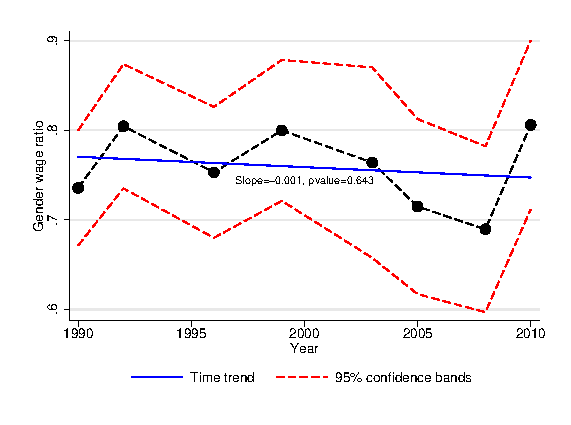
\includegraphics[width=.6\textwidth]{gender_wage_ratio}
	\label{fig:gender_wage_ratio}
	\source{Author's calculations using the China Health and Nutrition Survey.}
\end{figure}

In figure \ref{fig:skill_premium}, I plot the results I get for the skill premium on hourly wages. Like \cite{getao14}, I get a marked increase in the skill premium, although for 1990 the skill premium seems too low. To get this figure I also control for age and province.

\begin{figure}[hp]
	\centering
	\caption{Skill distribution for Chinese people aged 20-35, 1990-2010}\label{fig:skill_premium}
	\subfloat[Males]{\includegraphics[width=.6\textwidth]{skill_premium_men}}
	\\
	\subfloat[Females]{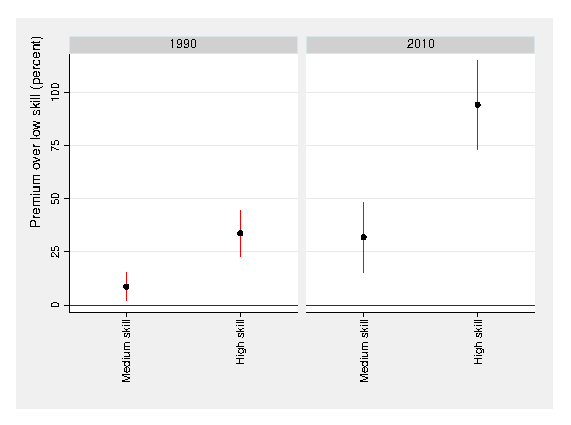
\includegraphics[width=.6\textwidth]{skill_premium_women}}
	\source{Author's calculations using the China Health and Nutrition Survey.}
	\note{skill levels are defined based on educational attainment (highest grade attained). Low skill individuals are those with primary or less, medium skill are those with middle-high school and high skill those with some college or more.}
\end{figure}


\subsection*{Three measures of assortative mating}

For the first measure, I regress wife's education level on her husband's:

\begin{align*}
EDU_{my}^w = \alpha + \beta\times EDU_{my}^h+\sum_{t\in T} \gamma_t\times EDU_{my}^h\times YEAR_{ty}+\sum_{t\in T}\theta_t\times YEAR_{ty}+\epsilon_{my}
\end{align*}

In the specification above, $EDU_{mw}^y$ and $EDU_{mh}^y$ represent wife's and husband's years of education in marriage $m$ and year $y$, and $YEAR_{ty}$ is a time dummy that takes the value of 1 when $t=y$ and 0 otherwise, whith $T = \{1992,1996,1999,2003,2005,2008,2010\}$. The coefficient $\beta$ measures the correlation between wife's and husband's education in the base year (1990), the $\theta_t$'s control for the secular rise in education. I am interested in the $\gamma_t$'s which measure the difference between wife and husband's correlation in year $t$ and the baseline year. If $\gamma_t$ rises with $t$, there's evidence of increasing assortative mating over time.

For the next two measures, I collapse the levels of education into three categories: low skill (primary or less), medium skill (High school) and high skill (college).

The second measure of assortative mating I use is Kendall's $\tau$ rank correlation. A value of 1 means perfect positive rank correlation, that is, the man with the highest education level is married with the woman with the highest education level, the man with the second highest education level is married with the woman with the second highest education level and so forth. A value of -1 means the opposite, i.e perfect negative rank correlation. The closer Kendall's $\tau$ is to 1, the higher the assortative mating. I measure $\tau_t$ for $t\in \{1990,1992,1996,1999,2003,2005,2008,2010\}$. Again, if $\tau_t$ rises with $t$, this points to increasing assortative mating over time.

Finally, I compute a measure of assortative mating based on contingency tables, as the one shown in table \ref{tab:cont_tab_1990} for 1990. Each cell has two entries: the one on the left gives the observed fraction of married households with the combination of wife and husband's education for that row and column. The second gives the fraction of households there would be in that cell if matching was random. This is obtained by multiplying the total fraction of women in her education category (the sum of elements in that row) by the total fraction of men in his (the sum of elements in that column). The values along the diagonal are the fractions of marriages where both spouses have the same education level. To measure assortative mating, I take the sum along the diagonal for both the observed and random matches, and divide the first by the second. This is denoted $\Delta_t$, and I compute it again for $t\in \{1990,1992,1996,1999,2003,2005,2008,2010\}$. Values of $\Delta_t$ above 1 mean that there is positive assortative mating, as the observed fraction of matches in which spouses have the same education is larger than the one random matching would produce. Once more, if $\Delta_t$ rises with $t$, there's evidence of increasing assortative mating.

\begin{table}[htbp]
	\centering
	\caption{Contingency table for marriages in China, 1990}
	\begin{tabular}{lccrccrccrr}
		\toprule
		\multicolumn{1}{c}{\multirow{2}[4]{*}{Wife}} & \multicolumn{10}{c}{Husband} \\
		\cmidrule{2-11}      & \multicolumn{2}{c}{Low skill} &       & \multicolumn{2}{c}{Medium skill} &       & \multicolumn{2}{c}{High skill} &       & \multicolumn{1}{l}{Marginal} \\
		\midrule
		Low skill & \textbf{0.251} & \textbf{0.164} &       & 0.247 & 0.317 &       & 0.006 & 0.023 &       & 0.504 \\
		Medium skill & 0.074 & 0.153 &       & \textbf{0.371} & \textbf{0.294} &       & 0.023 & 0.021 &       & 0.468 \\
		High skill & 0.001 & 0.009 &       & 0.011 & 0.018 &       & \textbf{0.017} & \textbf{0.001} &       & 0.028 \\
		Marginal & \multicolumn{2}{c}{0.326} &       & \multicolumn{2}{c}{0.629} &       & \multicolumn{2}{c}{0.046} &       &  \\
		\bottomrule
		\bottomrule
	\end{tabular}
	\label{tab:cont_tab_1990}
	\source{Author's calculations using the China Health and Nutrition Survey.}
\end{table}

\section{Solution of the time allocation and home production problem} \label{sec:timeallocationappendix}

\subsection*{Single agents}

The problem of a single agent of sex $i\in\{f,m\}$ and type $z$ can be written as

\begin{align*}
U_S^i\left(z\right) = & \max_{c,l,h,e_q} u\left(c,l,G\left(h,e_q\right)\right) \\
& \text{subject to} \\
& c = \omega_i\left(z\right)\left(1-l-h\right)-p_e e_q
\end{align*}

the corresponding Lagrangian is

\begin{align*}
	\mathcal{L}: \frac{\sigma_c}{1-\sigma}c^{1-\sigma}+\frac{\sigma_l}{1-\sigma}l^{1-\sigma}+\frac{\sigma_g}{1-\sigma}\left[A_G\left[e_q^{1-\alpha_G}\right]h^{\alpha_G}\right]^{1-\sigma}+\lambda_i(z)\left[\omega_i\left(z\right)\left(1-l-h\right)-p_e e_q\right]
\end{align*} 

the first order conditions are given by

\begin{align}
	& \sigma_c c^{-\sigma}-\lambda_i(z) = 0 \implies c=\left(\frac{\sigma_c}{\lambda_i(z)}\right)^{\frac{1}{\sigma}} \tag{SFOC 1} \label{SFOC1} \\
	& \sigma_l l^{-\sigma}-\lambda_i(z)\omega_i(z) = 0 \implies l=\left(\frac{\sigma_l}{\lambda_i(z)\omega_i(z)}\right)^{\frac{1}{\sigma}} \tag{SFOC 2} \label{SFOC2} \\
	& \sigma_g g^{-\sigma}A_G\alpha_G \left[e_q^{1-\alpha_G}\right]h^{\alpha_G-1}-\lambda_i(z)\omega_i(z) = 0 \tag{SFOC 3} \label{SFOC3} \\
	& \sigma_g g^{-\sigma}A_G\left(1-\alpha_G\right)\left[e_q^{-\alpha_G}\right]h^{\alpha_G}-\lambda_i(z) p_e \tag{SFOC 4} \label{SFOC4}
\end{align}

from \ref{SFOC1} and \ref{SFOC2} we have derived demands for market goods and leisure. From \ref{SFOC3} and \ref{SFOC4} we can derive an expression for the ratio between home equipment use and housework

\begin{align*}
	& \frac{\sigma_g g^{-\sigma}A_G\alpha_G \left[e_q^{1-\alpha_G}\right]h^{\alpha_G-1}}{\omega_i(z)}=\frac{\sigma_g g^{-\sigma}A_G\left(1-\alpha_G\right)\left[e_q^{-\alpha_G}\right]h^{\alpha_G}}{p_e} \\
	\iff & x_i^e(z) \equiv \frac{e_q}{h} = \frac{\left(1-\alpha_G\right)\omega_i(z)}{\alpha_G p_e}  
\end{align*}

furthermore, the ratio of home production to housework can be expressed as a function of $x_i^e(z)$

\begin{align*}
	x_i^g(z) \equiv \frac{g}{h} = \frac{A_G\left[e_q^{1-\alpha_G}\right]h^{\alpha_G}}{h}=A_G\left(\frac{e_q}{h}\right)^{1-\alpha_G}=A_G \left[x_i^e(z)\right]^{1-\alpha_G}
\end{align*}

from \ref{SFOC3} we can derive an expression for the demand of home produced goods that is a function of $x_i^e(z)$ and the lagrange multiplier

\begin{align*}
	g = \left(\frac{\sigma_g}{\lambda_i(z) D_i(z)}\right)^{\frac{1}{\sigma}}
\end{align*}

where $D_i(z)=\frac{\omega_i(z)}{A_G \alpha_G \left[x_i^e(z)\right]^{1-\alpha_G}}$ is the effective marginal price of home goods. Moreover, $h=\frac{g}{x_i^g(z)}$ and $e_q = \frac{x_i^e(z) g}{x_i^g(z)}$.

Subsituting the expressions for $c$, $l$, $h$ and $e_q$ in the budget constraint

\begin{align*}
	\left(\frac{\sigma_c}{\lambda_i(z)}\right)^{\frac{1}{\sigma}}=\omega_i\left(z\right)\left[1-\left(\frac{\sigma_l}{\lambda_i(z)\omega_i(z)}\right)^{\frac{1}{\sigma}}-\frac{g}{x_i^g(z)}\right]-p_e\frac{x_i^e(z) g}{x_i^g(z)}
\end{align*}

substituting the expression for $g$, we can solve for the Lagrange multiplier

\begin{align*}
	& \left(\frac{\sigma_c}{\lambda_i(z)}\right)^{\frac{1}{\sigma}}=\omega_i\left(z\right)\left[1-\left(\frac{\sigma_l}{\lambda_i(z)\omega_i(z)}\right)^{\frac{1}{\sigma}}-\frac{\left(\frac{\sigma_g}{\lambda_i(z) D_i(z)}\right)^{\frac{1}{\sigma}}}{x_i^g(z)}\right]-p_e\frac{x_i^e(z) \left(\frac{\sigma_g}{\lambda_i(z) D_i(z)}\right)^{\frac{1}{\sigma}}}{x_i^g(z)} \\
	\implies & \lambda_i(z) = \left[\frac{\sigma_c^{\frac{1}{\sigma}}+\omega_i\left(z\right)\left(\frac{\sigma_l}{\omega_i(z)}\right)^{\frac{1}{\sigma}}+\frac{\omega_i\left(z\right)}{x_i^g(z)}\left(\frac{\sigma_g}{D_i(z)}\right)^{\frac{1}{\sigma}}+\frac{p_e x_i^e(z)}{x_i^g(z)}\left(\frac{\sigma_g}{D_i(z)}\right)^{\frac{1}{\sigma}}}{\omega_i(z)}\right]^\sigma
\end{align*}

notice that the above expressions for $x_i^g(z)$, $D_i(z)$, $x_i^e(z)$ (and thus $\lambda_i(z)$) depend only on parameters of the model. Thus, we have found a closed-form solution for the time allocation problem. This solution will be always interior for singles, as the marginal utilities of market goods consumption, leisure and home produced goods all go to infinity when paid work, leisure or housework time go to zero, respectively.

\subsection*{Married households}

The problem of a married household  with wife's type $z_f$ and husband's type $z_m$ can be written as

\begin{align*}
	& \max_{c_f,c_m,l_f,l_m,h_m,h_f,eq} \left\lbrace \chi_fu_f\left(c_f,l_f\right)+ \left(1-\chi_f\right)u_m\left(c_m,l_m\right)+\frac{\sigma_g}{1-\sigma}G\left[H\left(h_f,h_m\right),e_q\right]^{1-\sigma}\right\rbrace \\
	&\text{subject to} \\
	& c_f+c_m = \omega_f(z_f)\left(1-l_f-h_f\right)+\omega_m(z_m)\left(1-l_m-h_m\right)-p_e e_q
\end{align*}

the Lagrangian of this problem is

\begin{align*}
	& \mathcal{L} : \\ &\chi_f\left(\frac{\sigma_c}{1-\sigma}c_f+\frac{\sigma_l}{1-\sigma}l_f\right)+\left(1-\chi_f\right)\left(\frac{\sigma_c}{1-\sigma}c_m+\frac{\sigma_l}{1-\sigma}l_m\right)+\frac{\sigma_g}{1-\sigma}G\left[H\left(h_f,h_m\right),e_q\right]^{1-\sigma} \\
	& +\lambda(z_f,z_m)\left[\omega_f(z_f)\left(1-l_f-h_f\right)+\omega_m(z_m)\left(1-l_m-h_m\right)-p_e e_q-c_f-c_m\right]
\end{align*}

the first order conditions are

\begin{align}
& \chi_f \sigma_c c_f^{-\sigma}-\lambda(z_f,z_m) = 0 \implies c_f=\left(\frac{\chi_f \sigma_c}{\lambda(z_f,z_m)}\right)^{\frac{1}{\sigma}} \tag{MFOC 1} \label{MFOC1} \\
& \left(1-\chi_f\right)\sigma_c c_m^{-\sigma}-\lambda(z_f,z_m) = 0 \implies c_m=\left(\frac{\left(1-\chi_f\right)\sigma_c}{\lambda(z_f,z_m)}\right)^{\frac{1}{\sigma}} \tag{MFOC 2} \label{MFOC2} \\
& \chi_f\sigma_l l_f^{-\sigma}-\lambda(z_f,z_m)\omega_f(z_f) = 0 \implies l_f=\left(\frac{\chi_f\sigma_l}{\lambda(z_f,z_m)\omega_f(z)}\right)^{\frac{1}{\sigma}} \tag{MFOC 3} \label{MFOC3} \\
& \left(1-\chi_f\right)\sigma_l l_m^{-\sigma}-\lambda(z_f,z_m)\omega_m(z_m) = 0 \implies l_m=\left(\frac{\left(1-\chi_f\right)\sigma_l}{\lambda(z_f,z_m)\omega_m(z_m)}\right)^{\frac{1}{\sigma}} \tag{MFOC 4} \label{MFOC4} \\
& \sigma_g g^{-\sigma}G_h H_{h_f}-\lambda(z_f,z_m)\omega_f(z_f) = 0 \tag{MFOC 5} \label{MFOC5} \\
& \sigma_g g^{-\sigma}G_h H_{h_m}-\lambda(z_f,z_m)\omega_m(z_m) = 0 \tag{MFOC 6} \label{MFOC6} \\
& \sigma_g g^{-\sigma}G_{e_q}-\lambda(z_f,z_m) p_e \tag{MFOC 7} \label{MFOC7}
\end{align}

where

\begin{align*}
	G_h &= \frac{\partial G}{\partial h} = \alpha_G A_G\left[e_q^{1-\alpha_G}\right]h^{\alpha_G-1} = \alpha_G A_G \left[\frac{e_q}{h}\right]^{1-\alpha_G} \\
	G_{e_q} &= \frac{\partial G}{\partial e_q} = \left(1-\alpha_G\right) A_G\left[e_q^{-\alpha_G}\right]h^{\alpha_G} = \left(1-\alpha_G\right) A_G \left[\frac{e_q}{h}\right]^{-\alpha_G} \\
	H_{h_f} &=\frac{\partial H}{\partial h_f}=\frac{1}{1-\eta}\left[\eta_f h_f^{1-\eta}+\left(1-\eta_f\right)h_m^{1-\eta}\right]^{\frac{1}{1-\eta}-1}\left(1-\eta\right)\eta_f h_f^{-\eta} \\
	& = h^{\eta}\eta_f h_f^{-\eta} \\
	H_{h_m} &=\frac{\partial H}{\partial h_m} = h^{\eta}\left(\eta_f\right)h_m^{-\eta}.
\end{align*}

Now, define $x^g(z_f,z_m)\equiv\frac{g}{h}$, $x^e(z_f,z_m)\equiv\frac{e_q}{h_m}$, $x^f(z_f,z_m)\equiv\frac{h_f}{h_m}$ and $x^h(z_f,z_m)\equiv\frac{h}{h_m}$. From \ref{MFOC7}

\begin{align*}
	g = \left(\frac{\sigma_g G_{eq}}{\lambda(z_f,z_m) p_e}\right)^{\frac{1}{\sigma}}=\left[\frac{\sigma_g \left(1-\alpha_G\right)A_G\left(\frac{e_q}{h}\right)^{-\alpha_G}}{\lambda(z_f,z_m) p_e}\right]^{\frac{1}{\sigma}}
\end{align*}

since $\frac{e_q}{h}=\frac{x^e(z_f,z_m)}{x^h(z_f,z_m)}$, then

\begin{align*}
	g = \left[\frac{\sigma_g \left(1-\alpha_G\right)A_G\left(\frac{x^e(z_f,z_m)}{x^h(z_f,z_m)}\right)^{-\alpha_G}}{\lambda(z_f,z_m) p_e}\right]^{\frac{1}{\sigma}}=\left(\frac{\sigma_g}{\lambda(z_f,z_m) D(z_f,z_m)}\right)^{\frac{1}{\sigma}}
\end{align*}

where $D = \frac{p_e\left(\frac{x^e(z_f,z_m)}{x^h(z_f,z_m)}\right)^{\alpha_G}}{A_G\left(1-\alpha_G\right)}$ is the effective marginal price of home goods.

From \ref{MFOC5} and \ref{MFOC6} we can derive a closed form expression for $x^f(z_f,z_m)$

\begin{align*}
	& \frac{\sigma_g g^{-\sigma}G_hH_{h_f}}{\omega_f(z_f)}=\frac{\sigma_g g^{-\sigma}G_hH_{h_m}}{\omega_m(z_m)} \\ \implies & \frac{H_{h_f}}{\omega_f(z_f)}=\frac{H_{h_m}}{\omega_m(z_m)} \\
    \implies & \frac{h^{\eta}\eta_f h_f^{-\eta}}{\omega_f(z_f)}=\frac{h^{\eta}\left(\eta_f\right)h_m^{-\eta}}{\omega_m(z_m)} \\
    \implies & x^f(z_f,z_m) \equiv \frac{h_f}{h_m} = \left[\frac{\eta_f \omega_m(z_m)}{\left(1-\eta_f\right)\omega_f(z_f)}\right]^{\frac{1}{\eta}} 
\end{align*}

using the expression above, we can derive one for $x^h(z_f,z_m)$. Substituting 

\begin{align*}
	h_f = \left[\frac{\eta_f \omega_m(z_m)}{\left(1-\eta_f\right)\omega_f(z_f)}\right]^{\frac{1}{\eta}}h_m
\end{align*}

into the expression for $h$

\begin{align*}
	& h = \left\lbrace \eta_f \left[\frac{\eta_f \omega_m(z_m)}{\left(1-\eta_f\right)\omega_f(z_f)}\right]^{\frac{1-\eta}{\eta}}h_m^{1-\eta}+\left(1-\eta_f\right)h_m^{1-\eta} \right\rbrace^{\frac{1}{1-\eta}} \\
	\implies & x^h(z_f,z_m) \equiv \frac{h}{h_m} = \left[\eta_f\left(\frac{\eta_f}{1-\eta_f} \frac{\omega_m(z_m)}{\omega_f(z_f)}\right)^{\frac{1-\eta}{\eta}}+1-\eta_f\right]^\frac{1}{1-\eta}.
\end{align*}

From \ref{MFOC6} and \ref{MFOC7} we can derive an expression for $x^e(z_f,z_m)$ that depends on $x^h(z_f,z_m)$ (for which we already have a closed form solution)

\begin{align*}
	& \frac{\sigma_g g^{-\sigma}G_h H_{h_m}}{\omega_m(z_m)} = \frac{\sigma_g g^{-\sigma}G_{e_q}}{p_e} \\
	\implies & \frac{\alpha_G A_G \left[\frac{e_q}{h}\right]^{1-\alpha_G} h^{\eta}\left(\eta_f\right)h_m^{-\eta}}{\omega_m(z_m)} = \frac{\left(1-\alpha_G\right) A_G \left[\frac{e_q}{h}\right]^{-\alpha_G}}{p_e} \\
	\implies & \frac{x^e(z_f,z_m)}{x^h(z_f,z_m)}x^h(z_f,z_m)^{\eta}=\frac{\left(1-\alpha_G\right)\omega_m(z_m)}{\alpha_G p_e \left(1-\eta_f\right)} \\
	\implies & x^e(z_f,z_m) = \frac{\left(1-\alpha_G\right)\omega_m(z_m)x^h(z_f,z_m)^{1-\eta}}{\alpha_G p_e \left(1-\eta_f\right)} 
\end{align*}

we derive also an expression for $x^g(z_f,z_m)$ that depends on $x^e(z_f,z_m)$ and $x^h(z_f,z_m)$

\begin{align*}
	& g = A_G\left(e_q^{1-\alpha_G}\right)h^{\alpha_G} = A_G x^e(z_f,z_m)^{1-\alpha_G} x^h(z_f,z_m)^{\alpha_G}h_m \\ \implies & x^g(z_f,z_m)\equiv \frac{g}{h_m} = A_G x^e(z_f,z_m)^{1-\alpha_G} x^h(z_f,z_m)^{\alpha_G}.
\end{align*}

We are almost ready to derive an expression for the Lagrange multiplier. We just have to notice that $h_m=\frac{g}{x^g(z_f,z_m)}$, $h_f=\frac{gx^f(z_f,z_m)}{x^g(z_f,z_m)}$ and $e_q=\frac{gx^e(z_f,z_m)}{x^g(z_f,z_m)}$, and substitute these along with the expressions for $c_f$, $c_m$, $l_f$, $l_m$ and $g$ in the budget constraint

\begin{align*}
	& \left(\frac{\chi_f \sigma_c}{\lambda(z_f,z_m)}\right)^{\frac{1}{\sigma}}+\left(\frac{\left(1-\chi_f\right)\sigma_c}{\lambda(z_f,z_m)}\right)^{\frac{1}{\sigma}}=\omega_f(z_f)\left[1-\left(\frac{\chi_f\sigma_l}{\lambda(z_f,z_m)\omega_f(z_f)}\right)^{\frac{1}{\sigma}}-\frac{gx^f(z_f,z_m)}{x^g(z_f,z_m)}\right] \\ & +\omega_m(z_m)\left[1-\left(\frac{\left(1-\chi_f\right)\sigma_l}{\lambda(z_f,z_m)\omega_m(z_m)}\right)^{\frac{1}{\sigma}}-\frac{g}{x^g(z_f,z_m)}\right]+p_e\frac{x^e(z_f,z_m) g}{x^g(z_f,z_m)}
\end{align*}

finally, the closed form expression for the Lagrange multiplier is

\begin{align*}
	\lambda(z_f,z_m) = \left(\frac{B(z_f,z_m)}{\omega_f(z_f)+\omega_m(z_m)}\right)^\sigma
\end{align*}
 
where

\begin{align*}
	B(z_f,z_m) & = \left(\chi_f \sigma_c\right)^{\frac{1}{\sigma}}+\left[\left(1-\chi_f\right) \sigma_c\right]^{\frac{1}{\sigma}}+\omega_f(z_f)\left(\frac{\chi_f \sigma_l}{\omega_f(z_h)}\right)^{\frac{1}{\sigma}}+\omega_m(z_m)\left[\frac{\left(1-\chi_f\right) \sigma_l}{\omega_m(z_m)}\right]^{\frac{1}{\sigma}} \\ & +\left(\frac{\sigma_g}{D(z_f,z_m)}\right)^{\frac{1}{\sigma}}\left[\frac{\omega_f(z_f)}{x^g(z_f,z_m)}x^f(z_f,z_m)+\frac{\omega_m(z_m)}{x^g(z_f,z_m)}+\frac{p_e x^e(z_f,z_m)}{x^g(z_f,z_m)}\right]
\end{align*}
 
Solutions may not always be interior for the married household problem. In particular, for some parameter configurations $h_f$, $h_m$, $n_f$ or $n_m$ could optimally be zero, i.e., there may be solutions in which one of the spouses doesn't do paid work or housework. Whenever solutions are not interior I rely on numerical methods to find the optimal quantities for married households.
 
\end{document}